% =========================================================
%  Chapter 8 — LEDs, Semiconductor Optical Amplifiers,
%              and the Laser Diode
%  Source: Dr. George's Lectures (Lecture 4)
%  Style: student-voice notes matching the personal style guide
% =========================================================

% ------------------------------------------------------------------
\section{Putting the Rate Equation to Work}
% ------------------------------------------------------------------

The carrier rate equation $dN/dt = J/(ed) - N/\tau - \Gamma G S$ is more than just a bookkeeping formula — it is the master equation that governs the entire family of semiconductor light sources. By solving it under different conditions and with different assumptions about the photon field, we recover the distinct operating regimes of three fundamentally different devices: the LED (spontaneous emission dominates, no optical feedback), the semiconductor optical amplifier (stimulated emission amplifies an external signal, no sustained oscillation), and the laser diode (stimulated emission dominates, optical feedback forces threshold and carrier clamping).

This chapter solves each case in turn, deriving the observable quantities — output power, bandwidth, gain saturation, threshold current, and the P--I characteristic — directly from the rate equation framework established in the previous chapter.

% ------------------------------------------------------------------
\section{The Light-Emitting Diode (LED)}
% ------------------------------------------------------------------

\subsection{Steady-State Output Power}

An LED operates far below the optical gain threshold — the photon density $S$ inside the device is negligibly small (no resonant cavity, no optical feedback), so the stimulated emission term $\Gamma G S$ in the carrier rate equation is completely negligible. At DC steady state, $dN/dt = 0$, and the rate equation reduces to a simple balance between injection and recombination:
\begin{equation*}
    \frac{J}{ed} = \frac{N}{\tau} \implies N = \frac{J\tau}{ed}
\end{equation*}

The photon generation rate per unit volume is the radiative fraction of the total recombination:
\begin{equation*}
    \frac{dS}{dt}\bigg|_\text{gen} = \frac{N}{\tau_r} = \frac{\tau}{\tau_r}\cdot\frac{J}{ed} = \eta_\text{int}\,\frac{J}{ed}
\end{equation*}

Multiplying by the photon energy $h\nu$ and the active volume $V = A \cdot d$ (where $A$ is the device area) converts the volumetric photon rate into total internal optical power:
\begin{keyresult}
    \begin{equation}
        P_\text{int} = \eta_\text{int}\,\frac{h\nu}{e}\,I
    \end{equation}
\end{keyresult}

This result has a clean physical interpretation: every electron injected has a probability $\eta_\text{int} = \tau/\tau_r$ of producing a photon, and each photon carries energy $h\nu$. The internal power scales linearly with current, limited only by the internal quantum efficiency.

\subsection{External Extraction Efficiency}

The internally generated photons face a second obstacle before escaping the chip: total internal reflection. A photon hitting the semiconductor-air interface at an angle beyond the critical angle $\theta_c$ is completely reflected back inside. The critical angle follows from Snell's law:
\begin{equation*}
    \sin\theta_c = \frac{n_a}{n_s}
\end{equation*}
where $n_s$ is the semiconductor refractive index ($n_s \approx 3.5$ for GaAs) and $n_a = 1$ To see how this escapes, consider an isotropic light source inside the semiconductor emitting power $P_0$ uniformly in all directions ($4\pi$ steradians). The power emitted per unit solid angle is $P_0/(4\pi)$. Light can only escape if it strikes the semiconductor-air interface within the escape cone defined by the critical angle $\theta_c$. The differential solid angle is $d\Omega = 2\pi\sin\theta\,d\theta$. The fraction of light emitted within this escape cone, accounting for the transmission probability $T(\theta)$, gives the external extraction efficiency:
\begin{equation*}
    \eta_\text{ext} = \frac{1}{4\pi}\int_0^{\theta_c} T(\theta)\cdot 2\pi\sin\theta\,d\theta
\end{equation*}

At normal incidence ($\theta = 0$), the reflection coefficient is given by the Fresnel reflection equation:
\begin{equation*}
    R(0) = \left(\frac{n_s - n_a}{n_s + n_a}\right)^2
\end{equation*}
By conservation of energy, the normal-incidence transmittance is $T(0) = 1 - R(0)$:
\begin{equation*}
    T(0) = 1 - \left(\frac{n_s - n_a}{n_s + n_a}\right)^2 = \frac{(n_s + n_a)^2 - (n_s - n_a)^2}{(n_s + n_a)^2} = \frac{4n_a n_s}{(n_a + n_s)^2}
\end{equation*}
For a high refractive index semiconductor ($n_s \gg n_a$), the critical angle $\theta_c$ is very small, meaning the escape cone is narrow. Over this narrow angle, the transmittance is approximately constant, $T(\theta) \approx T(0)$. Substituting this and evaluating the solid-angle integral:
\begin{equation*}
    \eta_\text{ext} = \frac{T(0)}{2}\int_0^{\theta_c}\sin\theta\,d\theta = \frac{T(0)}{2}(1 - \cos\theta_c)
\end{equation*}
Using the small-angle Taylor expansion for $\theta_c \ll 1$, we have $1 - \cos\theta_c \approx \theta_c^2/2 \approx \sin^2\theta_c/2$. Applying Snell's law ($\sin\theta_c = n_a/n_s$):
\begin{equation*}
    1 - \cos\theta_c \approx \frac{n_a^2}{2n_s^2}
\end{equation*}
Substituting this approximation back into the efficiency equation:
\begin{equation*}
    \eta_\text{ext} \approx \frac{T(0)}{2}\cdot\frac{n_a^2}{2n_s^2} = \frac{4n_a n_s}{(n_a+n_s)^2}\cdot\frac{n_a^2}{4n_s^2} = \frac{n_a^3}{n_s(n_a+n_s)^2}
\end{equation*}
which gives the closed-form result:
\begin{keyresult}
    \begin{equation}
        \eta_\text{ext} \approx \frac{n_a^3}{n_s(n_a + n_s)^2}
    \end{equation}
\end{keyresult}

\begin{figure}[H]
    \centering
    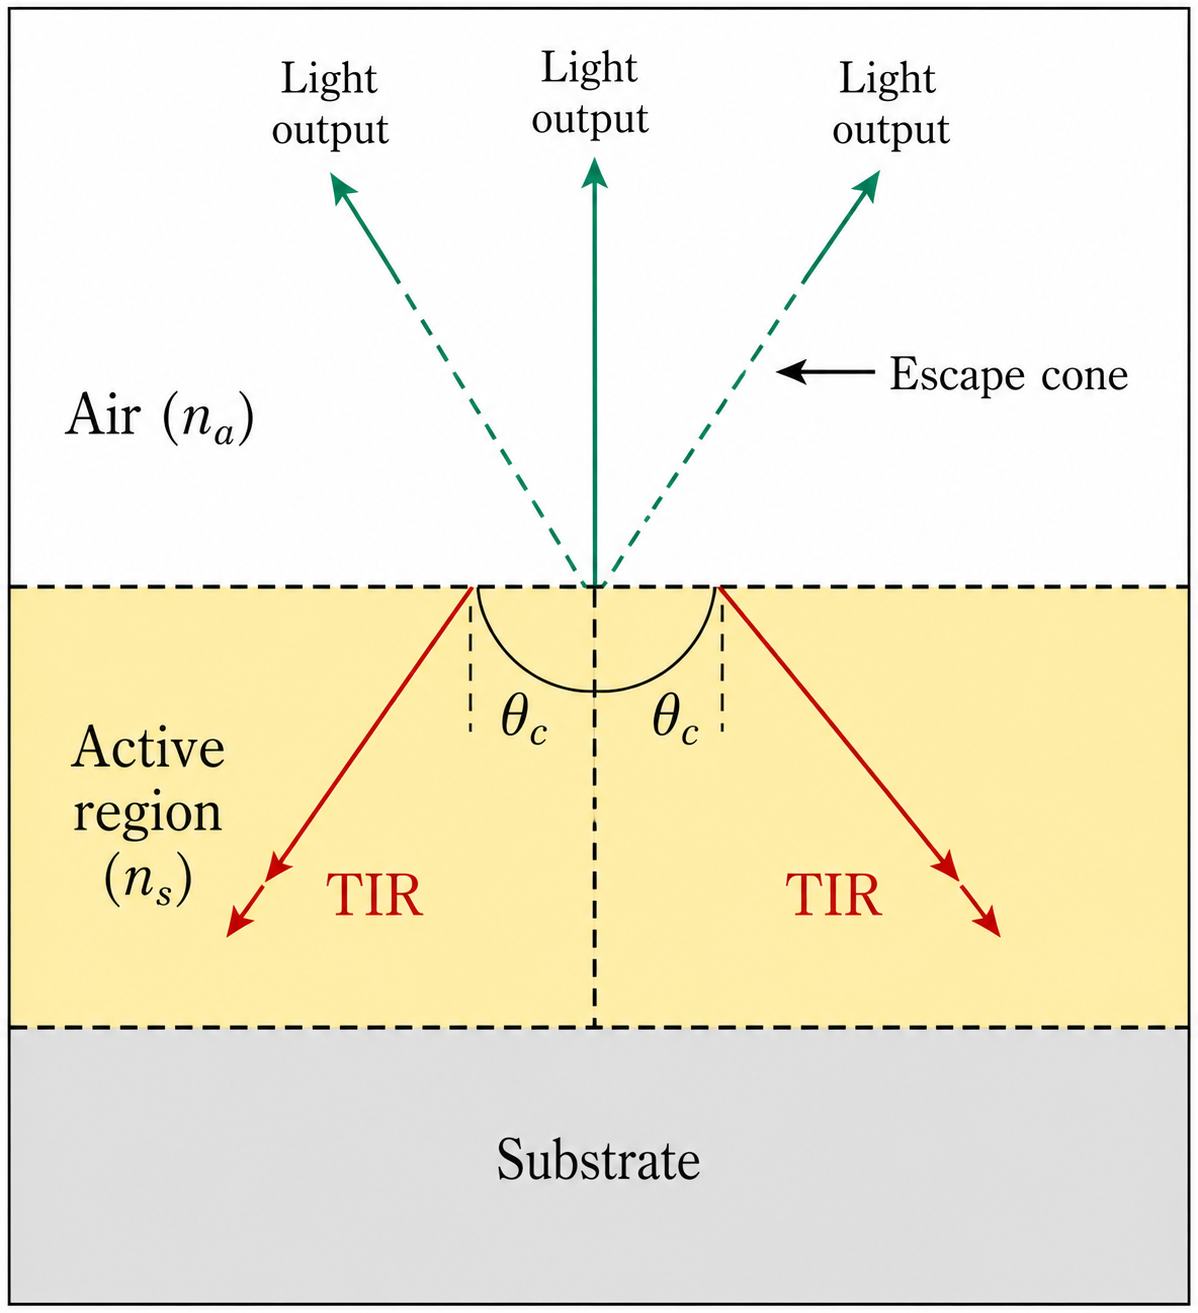
\includegraphics[width=0.6\textwidth]{Figures/Chapter 8/led_external_extraction_escape_cone_geometry.jpg}
    \caption{LED External Extraction: Escape Cone Geometry}
    \label{fig:led_external_extraction_escape_cone_geometry}
\end{figure}

For a GaAs LED ($n_s = 3.5$, $n_a = 1$): $\eta_\text{ext} \approx 1.4\%$. This brutally low number explains why practical LEDs invest heavily in geometric tricks — dome-shaped epoxy encapsulants, surface texturing, and chip shaping — to extract a larger fraction of the generated light.

\subsection{LED Responsivity}

Combining both efficiencies, the total output power is:
\begin{equation*}
    P_\text{out} = \eta_\text{ext}\,\eta_\text{int}\,\frac{h\nu}{e}\,I = R_\text{LED}\,I
\end{equation*}
where the \textbf{LED responsivity} is:
\begin{keyresult}
    \begin{equation}
        R_\text{LED} = \eta_\text{ext}\,\eta_\text{int}\,\frac{h\nu}{e} \quad [\text{W/A}]
    \end{equation}
\end{keyresult}

\begin{figure}[H]
    \centering
    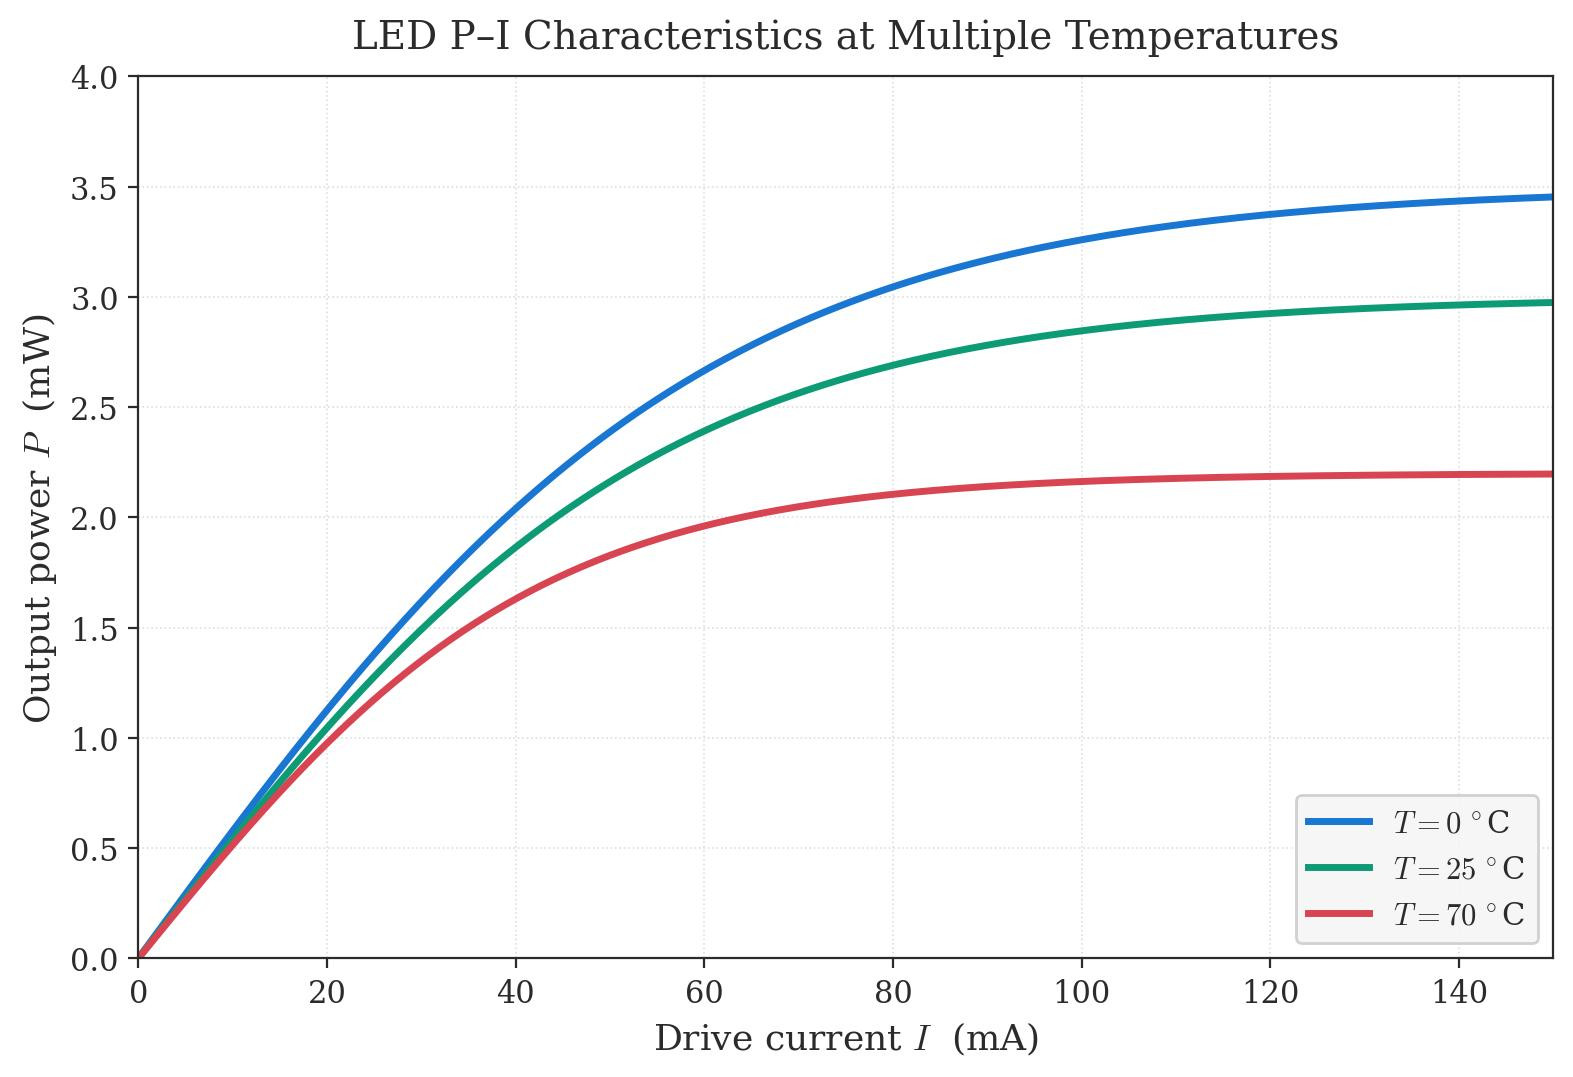
\includegraphics[width=0.6\textwidth]{Figures/Chapter 8/led_pi_temperature.jpg}
    \caption{LED P–I Characteristic at Multiple Temperatures}
    \label{fig:led_pi_temperature}
\end{figure}

The responsivity is the slope of the P--I curve. At low currents it is constant, but at high currents, Joule heating raises the junction temperature, increasing non-radiative recombination and reducing $\eta_\text{int}$. The P--I characteristic therefore sub-linearly rolls off at high drive currents — this rolloff is more severe at higher ambient temperatures, which is one reason LED datasheets always specify output power at a specific junction temperature.

\subsection{LED Emission Spectrum and Recombination Rate}

Under weak injection (where the quasi-Fermi levels remain within the bandgap and the Maxwell-Boltzmann approximation holds), the spontaneous emission rate per unit frequency interval $r_{sp}(\nu)$ is obtained by multiplying the joint density of states by the Boltzmann occupation probabilities. 
Note that while the energy joint density of states is $\rho_E(E) = \frac{\sqrt{2} m_r^{3/2}}{\pi^2 \hbar^3} \sqrt{E - E_g}$, we convert to a frequency scale via $\rho_\nu(\nu) = h \rho_E(h\nu)$. Because $h = 2\pi\hbar$, this cancels terms to yield the frequency density joint DOS:
\begin{equation*}
    \rho_\nu(\nu) = (2\pi\hbar) \frac{\sqrt{2} m_r^{3/2}}{\pi^2 \hbar^3} \sqrt{h\nu - E_g} = \frac{2\sqrt{2} m_r^{3/2}}{\pi \hbar^2} \sqrt{h\nu - E_g}
\end{equation*}
Multiplying by the spontaneous lifetime decay rate $1/\tau_r$ and the Boltzmann factor:
\begin{equation*}
    r_{sp}(\nu) = \frac{1}{\tau_r} \rho_\nu(\nu) \exp\!\left(-\frac{h\nu}{k_B T}\right) = \frac{1}{\tau_r} \left( \frac{2\sqrt{2} m_r^{3/2}}{\pi \hbar^2} \sqrt{h\nu - E_g} \right) \exp\!\left(-\frac{h\nu - E_g}{k_B T}\right) \exp\!\left(-\frac{E_g}{k_B T}\right)
\end{equation*}

This lineshape — a square-root rise above $E_g$ multiplied by a decaying exponential — has a peak frequency determined by differentiating with respect to $h\nu$ (or equivalently the kinetic energy variable $x = h\nu - E_g$). Differentiating $S(x) = \sqrt{x} e^{-x/k_B T}$:
\begin{equation*}
    \frac{dS}{dx} = \frac{1}{2\sqrt{x}} e^{-x/k_B T} - \frac{\sqrt{x}}{k_B T} e^{-x/k_B T} = 0 \implies \frac{1}{2\sqrt{x}} = \frac{\sqrt{x}}{k_B T} \implies x = \frac{k_B T}{2}
\end{equation*}
Substituting $x = h\nu_p - E_g$ yields the precise peak frequency:
\begin{keyresult}
    \begin{equation}
        h\nu_p = E_g + \frac{k_B T}{2}
    \end{equation}
\end{keyresult}
The peak sits exactly $k_BT/2$ above the bandgap. If we substitute this peak frequency back into the rate equation, the maximum spontaneous emission rate per unit frequency is:
\begin{equation*}
    r_{sp}(\nu_p) = \frac{2\sqrt{2} m_r^{3/2}}{\pi \hbar^2 \tau_r} \sqrt{\frac{k_B T}{2}} \exp\!\left(-\frac{1}{2}\right) \exp\!\left(-\frac{E_g}{k_B T}\right) = \frac{2 m_r^{3/2}}{\pi \hbar^2 \tau_r} \sqrt{\frac{k_B T}{e}} \exp\!\left(-\frac{E_g}{k_B T}\right)
\end{equation*}

More importantly, if we integrate this entire spectrum over all frequencies from $\nu = E_g/h$ to $\infty$, we obtain the total spontaneous emission rate per unit volume. We use the change of variables $u = \frac{h\nu - E_g}{k_B T} \implies d\nu = \frac{k_B T}{h}\,du = \frac{k_B T}{2\pi\hbar}\,du$:
\begin{align*}
    \int_{E_g/h}^\infty r_{sp}(\nu)\,d\nu &= \frac{2\sqrt{2}m_r^{3/2}}{\pi \hbar^2 \tau_r} \exp\!\left(-\frac{E_g}{k_B T}\right) \int_0^\infty \left( \sqrt{k_B T} \sqrt{u} \right) e^{-u} \left(\frac{k_B T}{2\pi\hbar}\,du\right) \\
    &= \frac{\sqrt{2}m_r^{3/2}}{\pi^2 \hbar^3 \tau_r} (k_B T)^{3/2} \exp\!\left(-\frac{E_g}{k_B T}\right) \int_0^\infty \sqrt{u}\,e^{-u}\,du
\end{align*}
Using the standard integral result $\int_0^\infty \sqrt{u}\,e^{-u}\,du = \frac{\sqrt{\pi}}{2}$:
\begin{equation*}
    \int_{E_g/h}^\infty r_{sp}(\nu)\,d\nu = \frac{\sqrt{2}m_r^{3/2}}{\pi^2 \hbar^3 \tau_r} (k_B T)^{3/2} \exp\!\left(-\frac{E_g}{k_B T}\right) \left(\frac{\sqrt{\pi}}{2}\right) = \frac{m_r^{3/2}}{\sqrt{2} \pi^{3/2} \hbar^3 \tau_r} (k_B T)^{3/2} \exp\!\left(-\frac{E_g}{k_B T}\right)
\end{equation*}

This exact quantum-mechanical integration is the physical foundation for the macroscopic recombination parameter $r$ (used in the rate $R = rnp$). Under equilibrium conditions, $np = n_i^2$. We write the intrinsic carrier concentration using the effective densities of states:
\begin{align*}
    n_i^2 &= N_c N_v \exp\!\left(-\frac{E_g}{k_B T}\right) \\
    &= \left( 2\left[\frac{2\pi m_e^* k_B T}{h^2}\right]^{3/2} \right) \left( 2\left[\frac{2\pi m_h^* k_B T}{h^2}\right]^{3/2} \right) \exp\!\left(-\frac{E_g}{k_B T}\right) \\
    &= 4 \left( \frac{2\pi \sqrt{m_e^* m_h^*} k_B T}{4\pi^2 \hbar^2} \right)^3 \exp\!\left(-\frac{E_g}{k_B T}\right) \\
    &= \frac{1}{2\pi^3 \hbar^6} (m_e^* m_h^*)^{3/2} (k_B T)^3 \exp\!\left(-\frac{E_g}{k_B T}\right)
\end{align*}
By equating the integrated spontaneous emission rate to the macroscopic rate $r n_i^2$:
\begin{equation*}
    r \left[ \frac{1}{2\pi^3 \hbar^6} (m_e^* m_h^*)^{3/2} (k_B T)^3 \exp\!\left(-\frac{E_g}{k_B T}\right) \right] = \frac{m_r^{3/2}}{\sqrt{2} \pi^{3/2} \hbar^3 \tau_r} (k_B T)^{3/2} \exp\!\left(-\frac{E_g}{k_B T}\right)
\end{equation*}
Solving for $r$ and using the reduced mass relation $m_r = \frac{m_e^* m_h^*}{m_e^* + m_h^*} \implies \frac{m_r}{m_e^* m_h^*} = \frac{1}{m_e^* + m_h^*}$:
\begin{align*}
    r &= \frac{m_r^{3/2}}{\sqrt{2}\pi^{3/2}\hbar^3 \tau_r (k_B T)^{3/2}} \cdot \frac{2\pi^3 \hbar^6}{(m_e^* m_h^*)^{3/2}} \\
    &= \frac{\sqrt{2}\pi^{3/2}\hbar^3}{\tau_r (k_B T)^{3/2}} \left( \frac{m_r}{m_e^* m_h^*} \right)^{3/2} \\
    &= \frac{\sqrt{2}\pi^{3/2}\hbar^3}{(m_e^* + m_h^*)^{3/2}} \frac{1}{(k_B T)^{3/2}\tau_r}
\end{align*}
yielding the final result:
\begin{keyresult}
    \begin{equation}
        r = \frac{\sqrt{2}\pi^{3/2}\hbar^3}{(m_e^* + m_h^*)^{3/2}} \frac{1}{(k_B T)^{3/2}\tau_r}
    \end{equation}
\end{keyresult}
This elegantly links a macroscopic device parameter ($r$) directly to the microscopic quantum mechanics ($m_e^*$, $m_h^*$, $\hbar$).

The FWHM of the spectrum in frequency is:
\begin{equation*}
    \Delta\nu_\text{FWHM} = \frac{1.8\,k_BT}{h}
\end{equation*}

Converting to wavelength bandwidth using $\Delta\lambda = (\lambda^2/c)\Delta\nu$, for a GaAs LED at $T = 300\,\text{K}$ this gives $\Delta\lambda \approx 40\,\text{nm}$ centred near $\lambda \approx 870\,\text{nm}$. This broad, incoherent spectrum (compared to the sub-nanometre linewidth of a laser diode) is the fundamental optical signature of spontaneous emission — no two photons are produced with a correlated phase.

\begin{figure}[H]
    \centering
    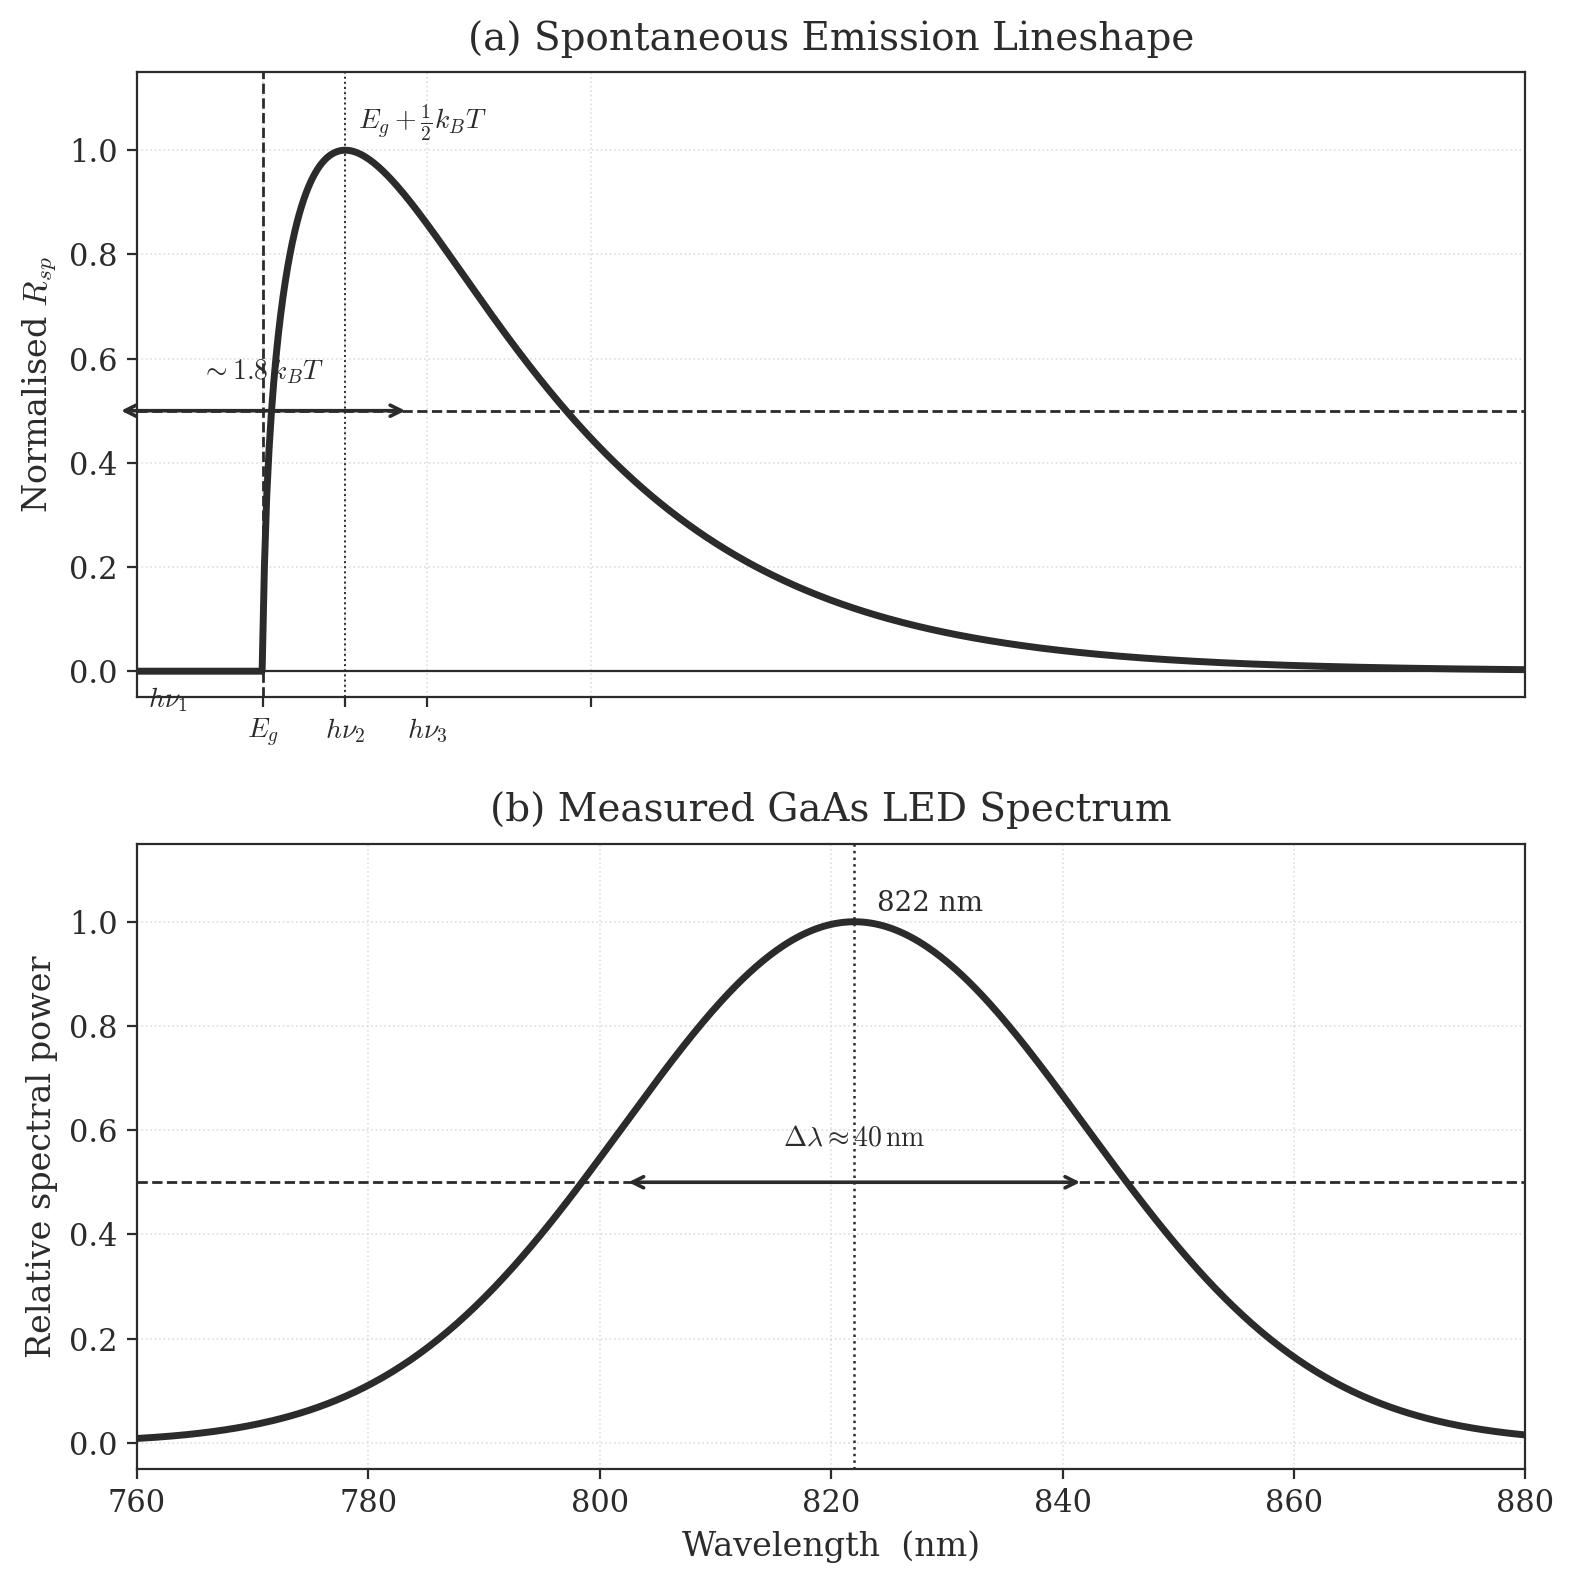
\includegraphics[width=0.7\textwidth]{Figures/Chapter 8/led_emission_spectrum.jpg}
    \caption{LED Emission Spectrum (Weak-Injection Lineshape)}
    \label{fig:led_emission_spectrum}
\end{figure}

\subsection{LED AC Modulation and Rise Time Dynamics}

To use an LED in a communications link, we must understand its transient and AC response. If we modulate the LED with a sinusoidal drive current $I(t) = I_b + I_m e^{j\omega_m t}$ superimposed on a DC bias $I_b$, the carrier density responds as $N(t) = N_b + N_m e^{j\omega_m t}$.

Substituting this into the carrier rate equation $dN/dt = I/(eV) - N/\tau$ and separating the DC and AC components yields two equations:
\begin{equation*}
    0 = \frac{I_b}{eV} - \frac{N_b}{\tau} \implies N_b = \frac{\tau I_b}{eV}
\end{equation*}
\begin{equation*}
    j\omega_m N_m = \frac{I_m}{eV} - \frac{N_m}{\tau} \implies N_m = \frac{\tau I_m / eV}{1 + j\omega_m\tau}
\end{equation*}

Because the optical output power $P(t)$ is directly proportional to the carrier density $N(t)$, the AC modulation index $m_n$ of the photon output is the magnitude of the AC carrier density divided by the DC carrier density. Taking the magnitude of the complex AC density $N_m$:
\begin{equation*}
    |N_m| = \frac{\tau I_m / eV}{\sqrt{1 + (\omega_m\tau)^2}}
\end{equation*}
Taking the ratio $|N_m|/N_b$ yields:
\begin{keyresult}
    \begin{equation}
        m_n = \frac{|N_m|}{N_b} = \frac{\frac{\tau I_m / eV}{\sqrt{1 + (\omega_m\tau)^2}}}{\frac{\tau I_b}{eV}} = \frac{I_m}{I_b \sqrt{1 + (\omega_m\tau)^2}}
    \end{equation}
\end{keyresult}
Furthermore, the denominator $1 + j\omega_m\tau$ is a complex number with phase angle $\arg(1 + j\omega_m\tau) = \tan^{-1}(\omega_m\tau)$. Because this term is in the denominator of $N_m$, it introduces a phase lag $\theta$ between the injected AC current and the resulting optical AC output:
\begin{keyresult}
    \begin{equation}
        \theta = \arg(N_m) = -\tan^{-1}(\omega_m\tau)
    \end{equation}
\end{keyresult}

The 3\,dB modulation bandwidth — the frequency $f_{3\text{dB}}$ at which the AC optical power drops by half ($1/\sqrt{2}$ in amplitude) — occurs when $\omega_m \tau = 1$:
\begin{equation*}
    f_{3\text{dB}} = \frac{1}{2\pi\tau}
\end{equation*}
This reveals a fundamental design tension: maximizing bandwidth requires a short carrier lifetime $\tau$, but shortening $\tau$ (often by increasing non-radiative recombination) drastically reduces the internal quantum efficiency $\eta_{\text{int}}$.

Finally, let us examine the large-signal time-domain response. If we apply an abrupt current step $I(t) = I_o u(t)$, the carrier rate equation is a simple first-order ODE. The optical power rises exponentially:
\begin{equation*}
    P(t) = P_o \left( 1 - e^{-t/\tau} \right)
\end{equation*}
The standard metric for switching speed is the 10-90\% rise time $t_{\text{rise}}$. We find the times $t_{10}$ and $t_{90}$ by setting $P(t)/P_o$ to $0.1$ and $0.9$:
\begin{align*}
    1 - e^{-t_{10}/\tau} & = 0.1 \implies t_{10} = \tau \ln(10/9) \\
    1 - e^{-t_{90}/\tau} & = 0.9 \implies t_{90} = \tau \ln(10)
\end{align*}
Subtracting these gives the exact rise time:
\begin{keyresult}
    \begin{equation}
        t_{\text{rise}} = t_{90} - t_{10} = \tau \ln(9) \approx 2.2\tau
    \end{equation}
\end{keyresult}
Because we just established that $f_{3\text{dB}} = 1/(2\pi\tau)$, we can elegantly link the time-domain and frequency-domain speeds: $t_{\text{rise}} \approx \frac{2.2}{2\pi f_{3\text{dB}}} = \frac{0.35}{f_{3\text{dB}}}$.

\subsection{LED for Illumination: Luminous Efficacy}

In lighting applications, the relevant figure of merit is not watts of optical power but lumens of luminous flux — how much light the human eye perceives. The luminous flux from a monochromatic source at wavelength $\lambda$ is:
\begin{equation*}
    \Phi_\lambda = P(\lambda) \times 633\,\text{lm/W} \times V(\lambda)
\end{equation*}
where $V(\lambda)$ is the photopic luminosity function (the eye's relative sensitivity), normalised to unity at $\lambda = 555\,\text{nm}$ (peak green sensitivity). The overall \textbf{luminous efficacy}:
\begin{equation*}
    \eta_{LE} = \frac{1}{V}\int\eta_\text{ext}\,\eta_\text{int}\,\frac{hc}{q\lambda} \times 633 \times V(\lambda)\,d\lambda
\end{equation*}
accounts for both the electrical-to-photon conversion and the photon-to-lumens conversion by integrating over the emission spectrum weighted by the eye's response.

\begin{figure}[H]
    \centering
    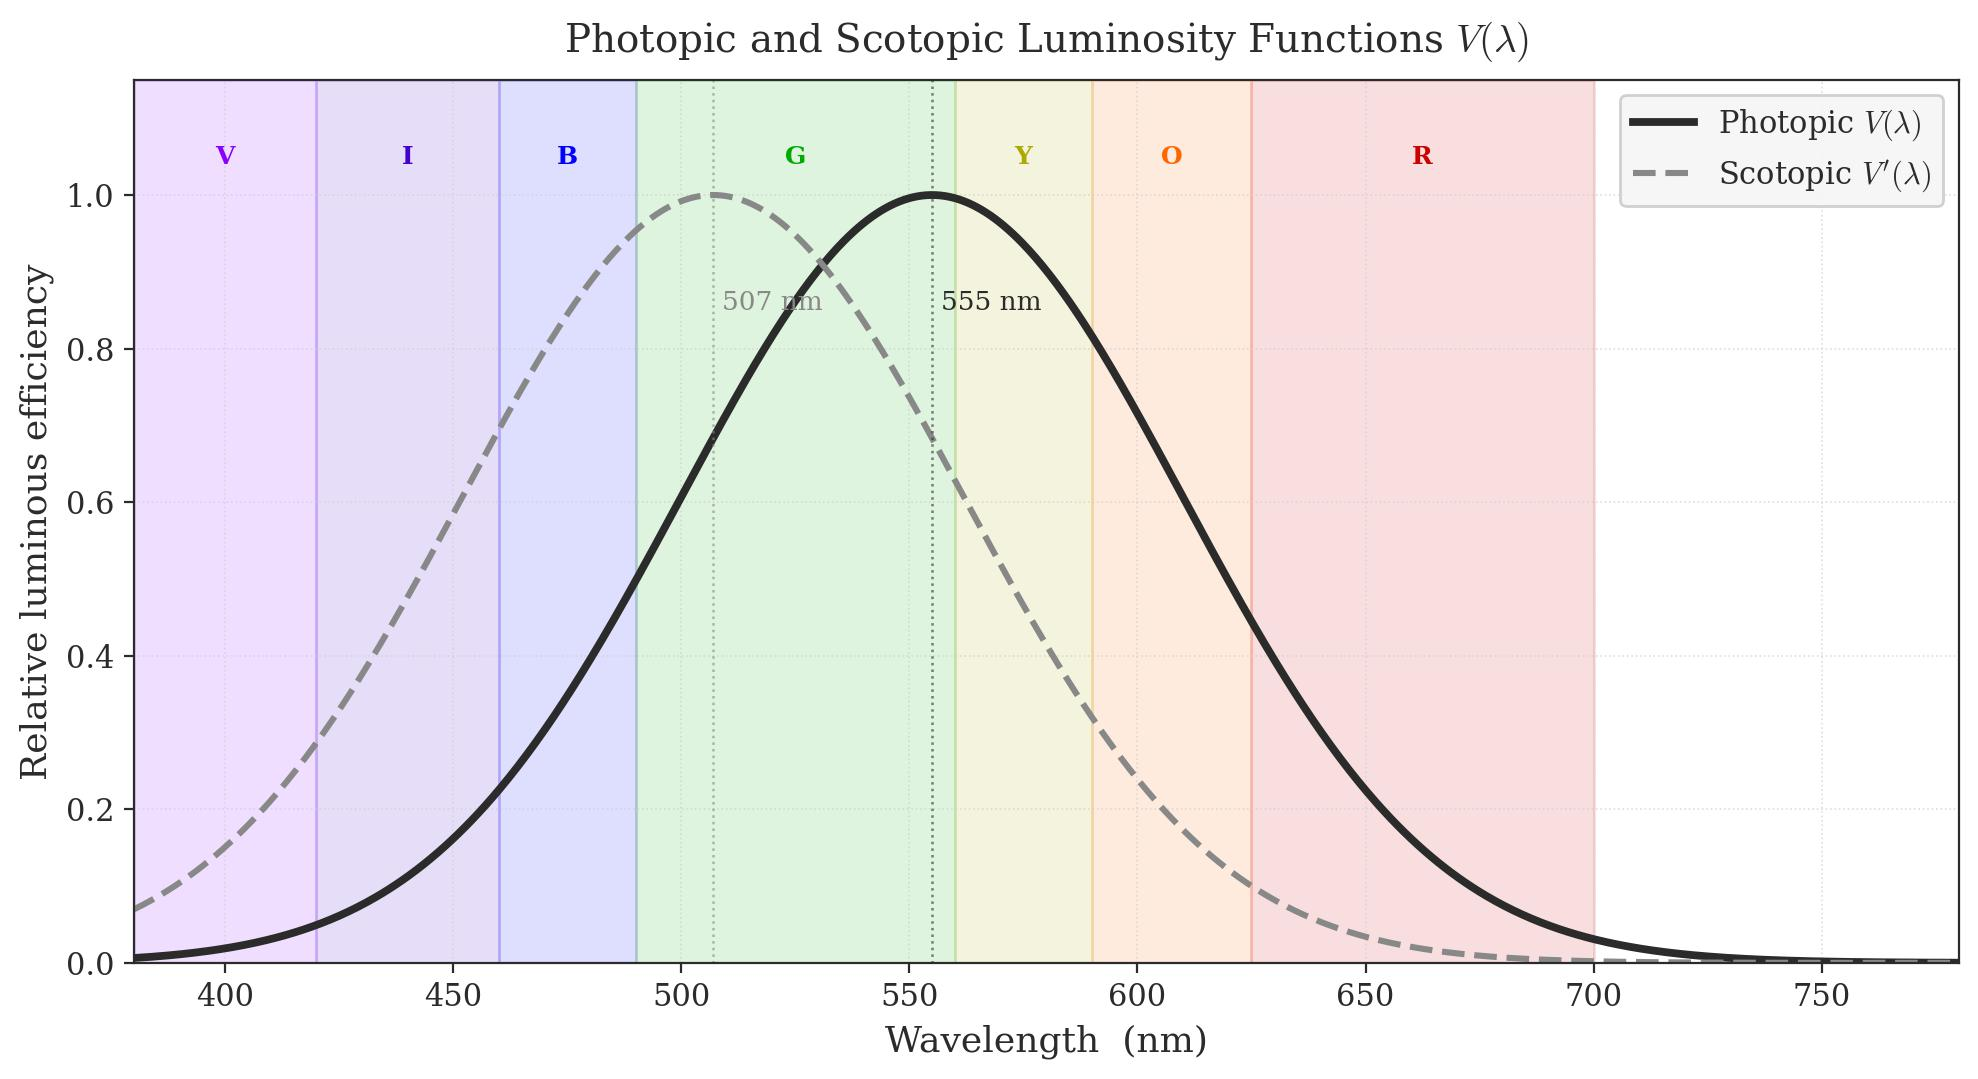
\includegraphics[width=0.6\textwidth]{Figures/Chapter 8/luminosity_functions.jpg}
    \caption{Photopic and Scotopic Luminosity Functions $V(\lambda)$}
    \label{fig:luminosity_functions}
\end{figure}

% ------------------------------------------------------------------
\section{The Semiconductor Optical Amplifier (SOA)}
% ------------------------------------------------------------------

\subsection{Degenerate Quasi-Fermi Separations and Positive Gain Bandwidth}

Before calculating the amplification factor, we must first determine the spectral window over which the SOA can actually provide positive gain. Net gain requires the Bernard-Duraffourg condition to be strictly satisfied: $E_g < h\nu < E_{fc} - E_{fv}$. Thus, the absolute maximum positive gain bandwidth is set by the separation of the quasi-Fermi levels.

In a heavily pumped SOA, the injected carrier density $\Delta n$ is so massive that the semiconductor becomes strongly degenerate. To find the quasi-Fermi levels, we approximate the Fermi-Dirac distribution at $T=0\text{ K}$ as a perfect step function. The carrier density is found by integrating the 3D density of states $\rho_c(E)$ from the conduction band edge $E_c$ up to the electron quasi-Fermi level $E_{fc}$:
\begin{equation*}
    n = \int_{E_c}^{E_{fc}} \frac{1}{2\pi^2} \left( \frac{2m_e^*}{\hbar^2} \right)^{3/2} \sqrt{E - E_c} \,dE = \frac{1}{3\pi^2} \left( \frac{2m_e^*}{\hbar^2} \right)^{3/2} (E_{fc} - E_c)^{3/2}
\end{equation*}

Solving this directly for the electron quasi-Fermi level $E_{fc}$ (and doing the symmetric derivation for holes) yields:
\begin{keyresult}
    \begin{equation}
        E_{fc} = E_c + (3\pi^2)^{2/3} \frac{\hbar^2}{2 m_e^*} (n)^{2/3} \qquad \text{and} \qquad E_{fv} = E_v - (3\pi^2)^{2/3} \frac{\hbar^2}{2 m_h^*} (p)^{2/3}
    \end{equation}
\end{keyresult}

If we subtract $E_{fv}$ from $E_{fc}$ to find the total separation, and recognize that under strong injection $n \approx p \approx \Delta n$, we find:
\begin{equation*}
    E_{fc} - E_{fv} = E_g + (3\pi^2)^{2/3} \frac{\hbar^2}{2} \left( \frac{1}{m_e^*} + \frac{1}{m_h^*} \right) (\Delta n)^{2/3} = E_g + (3\pi^2)^{2/3} \frac{\hbar^2}{2m_r} (\Delta n)^{2/3}
\end{equation*}
where $m_r$ is the reduced mass. The positive gain bandwidth $BW$ in Hz is the difference between the maximum amplifiable photon energy ($E_{fc}-E_{fv}$) and the minimum amplifiable photon energy ($E_g$), divided by Planck's constant $h$:
\begin{keyresult}
    \begin{equation}
        BW = \frac{(E_{fc}-E_{fv}) - E_g}{h} = (3\pi^2)^{2/3}\frac{h}{8\pi^2 m_r}(\Delta n)^{2/3}
    \end{equation}
\end{keyresult}
This elegantly proves that the optical amplification bandwidth of an SOA expands proportionally to $\Delta n^{2/3}$. More injected carriers physically push the quasi-Fermi levels deeper into the bands, widening the spectral window available for amplification.

\subsection{Small-Signal Amplification}

An SOA is a forward-biased semiconductor heterostructure with anti-reflection coatings on both facets, so that the photon density never builds up enough to sustain oscillation. An external optical signal enters one facet, is amplified by stimulated emission as it propagates through the gain medium, and exits the other facet with higher power.

\begin{figure}[H]
    \centering
    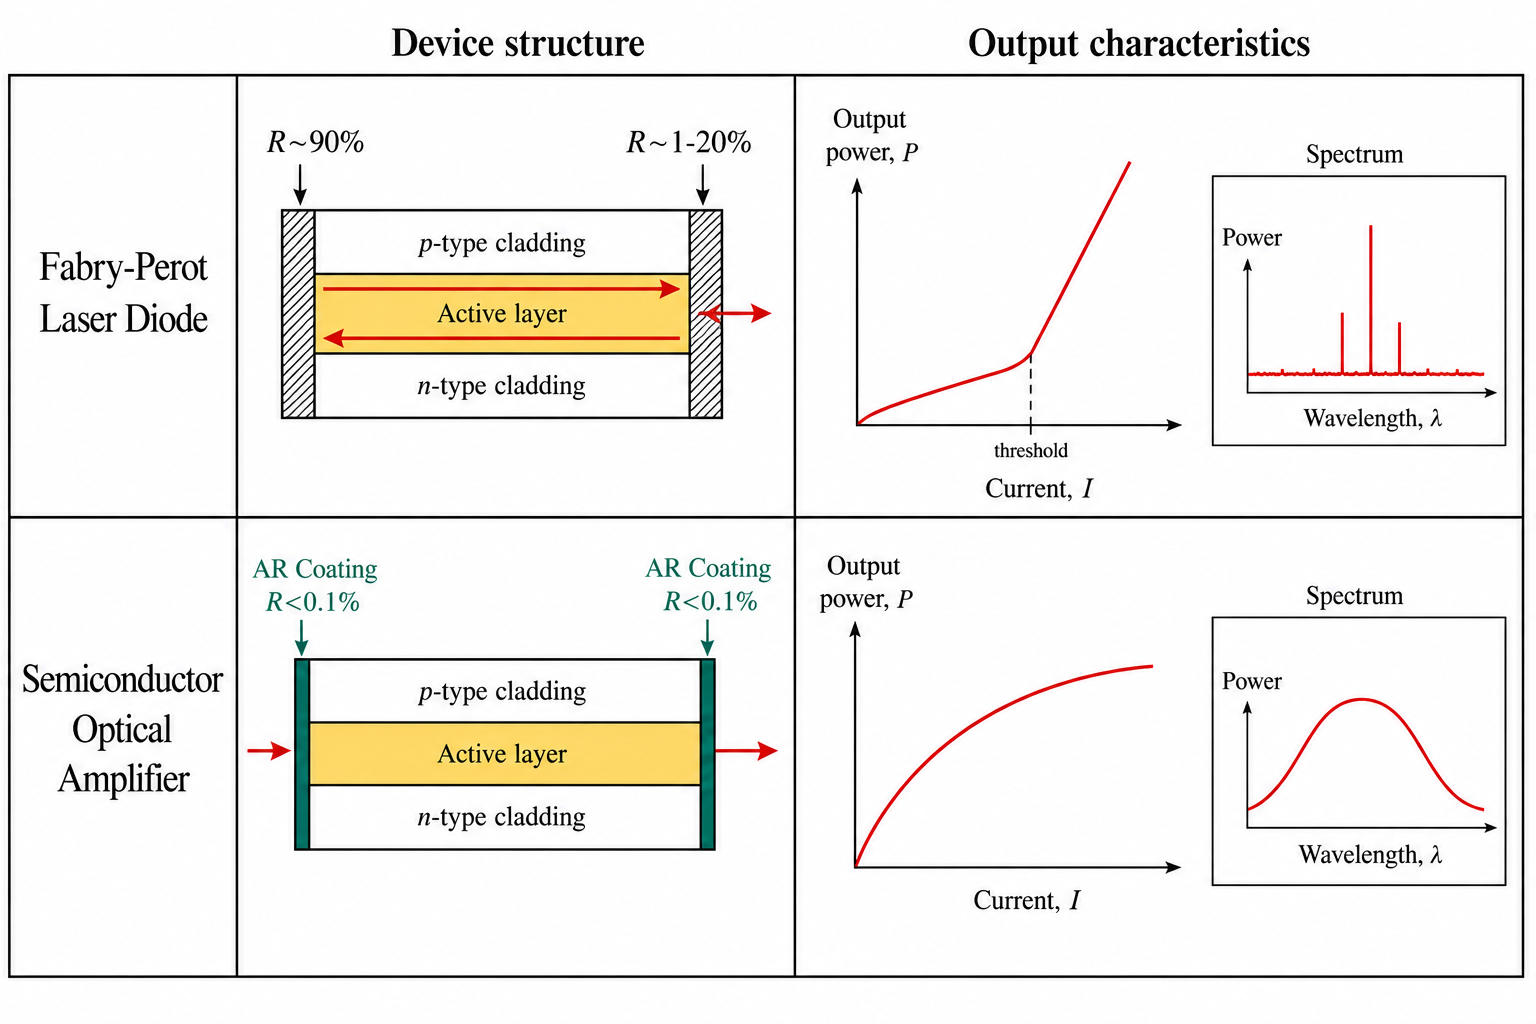
\includegraphics[width=0.7\textwidth]{Figures/Chapter 8/soa_vs_laser_diode_structure_and_output_characteristics.jpg}
    \caption{SOA vs. Laser Diode: Structure and Output Characteristics}
    \label{fig:soa_vs_laser_diode_structure_and_output_characteristics}
\end{figure}

In the small-signal regime, the input photon density $S$ is negligible compared to the carrier density, so the injected current pins the carrier density $N$ at its unsaturated value. The photon density then grows exponentially along the propagation direction $z$:
\begin{equation*}
    S(z) = S(0)\exp\!\left[\Gamma B(N - N_\text{tr})\,\frac{z}{v_g}\right]
\end{equation*}

Converting the exponential argument using $G = v_g\,\gamma_m = v_g B(N - N_\text{tr})$ gives the intensity amplification factor $\mathcal{G} = S_\text{out}/S_\text{in} = \exp(G_0 L)$, where $G_0 = \Gamma B(N - N_\text{tr})$ is the unsaturated gain coefficient and $L$ is the device length.

\subsection{Gain Saturation}

When the input power is large enough that the photon density $S$ becomes comparable to the carrier density, stimulated emission depletes the inversion. To quantify this, we set the carrier rate equation to zero at steady-state:
\begin{equation*}
    \frac{dN}{dt} = \frac{J}{ed} - \frac{N}{\tau} - \Gamma G S = 0
\end{equation*}
Expressing the carrier density in terms of the deviation from transparency $(N - N_\text{tr})$:
\begin{equation*}
    \frac{J}{ed} - \frac{N - N_\text{tr} + N_\text{tr}}{\tau} - \Gamma B(N - N_\text{tr}) S = 0 \implies \left(\frac{J}{ed} - \frac{N_\text{tr}}{\tau}\right) - (N - N_\text{tr})\left(\frac{1}{\tau} + \Gamma B S\right) = 0
\end{equation*}
Solving for $(N - N_\text{tr})$:
\begin{equation*}
    N - N_\text{tr} = \frac{\frac{J}{ed} - \frac{N_\text{tr}}{\tau}}{\frac{1}{\tau} + \Gamma B S} = \frac{\tau\left(\frac{J}{ed} - \frac{N_\text{tr}}{\tau}\right)}{1 + \Gamma B \tau S} = \frac{\Delta N_0}{1 + \Gamma B \tau S}
\end{equation*}
where $\Delta N_0 \equiv \tau\left(\frac{J}{ed} - \frac{N_\text{tr}}{\tau}\right)$ is the unsaturated population inversion.
Next, we relate the photon density $S$ to the optical power $P$ flowing through the waveguide mode. The cross-sectional area of the optical mode is $A_\text{mode} = A/\Gamma$. The optical power is the energy density $S \cdot h\nu$ multiplied by the group velocity $v_g$ and the mode area:
\begin{equation*}
    P = S \cdot h\nu \cdot v_g \cdot A_\text{mode} = \frac{S h\nu v_g A}{\Gamma} \implies S = \frac{\Gamma P}{v_g h\nu A}
\end{equation*}
Substituting this expression for $S$ into the denominator:
\begin{equation*}
    N - N_\text{tr} = \frac{\Delta N_0}{1 + \Gamma B \tau \left(\dfrac{\Gamma P}{v_g h\nu A}\right)} = \frac{\Delta N_0}{1 + \dfrac{P}{P_s}}
\end{equation*}
where we define the saturation power as $P_s \equiv \frac{v_g h\nu A}{\Gamma B \tau}$. The saturated material gain coefficient $g = B(N-N_\text{tr})$ then becomes:
\begin{keyresult}
    \begin{equation}
        g = \frac{g_0}{1 + P/P_s}, \qquad P_s = \frac{v_g h\nu A}{\Gamma B \tau}
    \end{equation}
\end{keyresult}
where $g_0 = B \Delta N_0$ is the unsaturated gain.

This homogeneous saturation form — gain compressing inversely with optical power — is the universal behaviour of any gain medium where stimulated emission depletes the inversion that feeds it. Integrating the propagation equation $dP/dz = g\,P$ through the device gives the transcendental implicit equation:
\begin{equation*}
    \ln\!\frac{P_\text{out}}{P_\text{in}} + \frac{P_\text{out} - P_\text{in}}{P_s} = g_0\,L
\end{equation*}

The 3\,dB gain compression point — where the total amplified power equals $P_s \ln 2$ — marks the boundary of the linear amplification regime. Beyond this point, the gain compresses rapidly and the amplifier distorts the signal.

\begin{figure}[H]
    \centering
    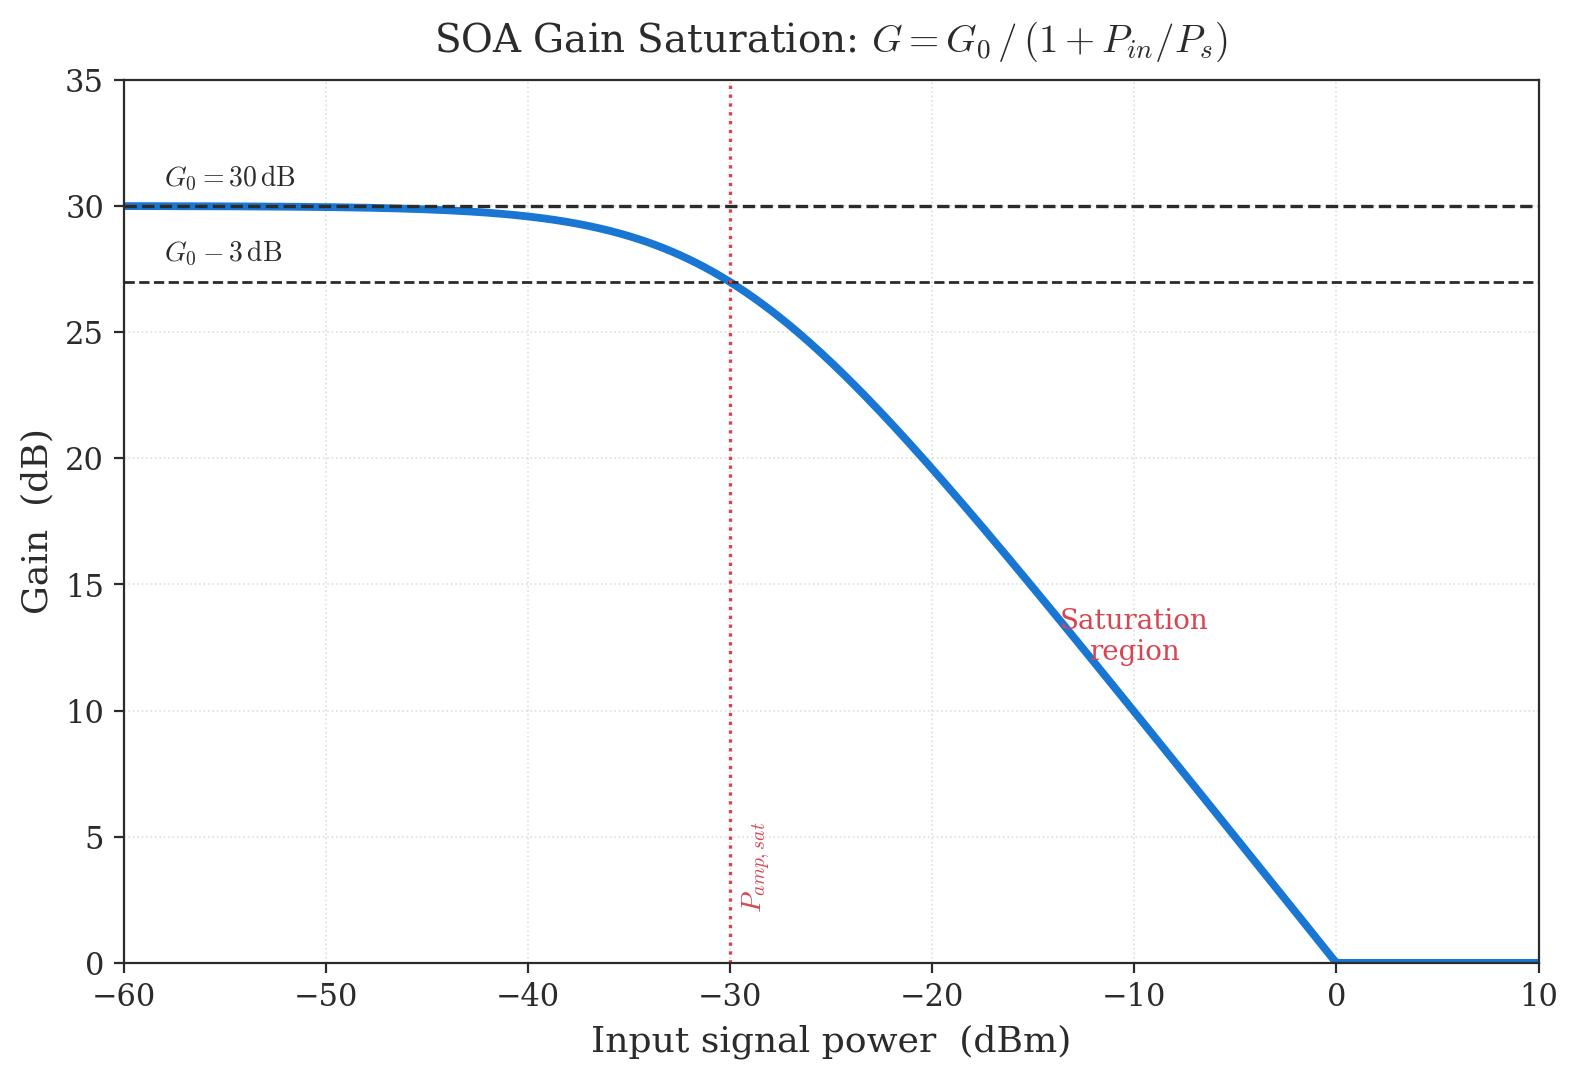
\includegraphics[width=0.6\textwidth]{Figures/Chapter 8/soa_gain_saturation.jpg}
    \caption{SOA Gain Saturation: Gain vs. Input Signal Power}
    \label{fig:soa_gain_saturation}
\end{figure}

\subsection{Noise Figure}

Any amplifier that adds spontaneous emission to the signal degrades its signal-to-noise ratio. The noise figure of the SOA is defined as:
\begin{equation*}
    F_n = \frac{(\text{SNR})_\text{in}}{(\text{SNR})_\text{out}}
\end{equation*}

For an SOA with internal loss $\alpha_\text{int}$ per unit length and total intensity gain $\mathcal{G}$:
\begin{keyresult}
    \begin{equation}
        F_n = 2\!\left(\frac{N}{N - N_\text{tr}}\right)\!\left(\frac{\mathcal{G}}{\mathcal{G} - \alpha_\text{int}L}\right)
    \end{equation}
\end{keyresult}

In the high-gain limit ($\mathcal{G} \gg 1$) with negligible internal loss, the noise figure approaches $F_n \to 2$ (equivalently, 3\,dB). This quantum-limited noise floor is set by amplified spontaneous emission (ASE): even with perfect population inversion, every amplification event is accompanied by some probability of spontaneous emission into the signal mode, adding shot noise. This 3\,dB quantum limit is fundamental and cannot be beaten by any linear optical amplifier — it is the optical analogue of the $kT$ thermal noise floor in electronic amplifiers.

\subsection{Polarisation Dependence and FP vs.\ TWA}

The rectangular cross-section of a standard SOA waveguide confines TE and TM polarisation modes differently, giving different confinement factors $\Gamma_\text{TE} \neq \Gamma_\text{TM}$. This makes the TE gain systematically higher than the TM gain by several dB at high input powers — a significant limitation for polarisation-diverse fibre-optic systems.

When facet reflectivities are non-zero (an SOA without perfect anti-reflection coatings), the device behaves as a Fabry-Pérot amplifier with frequency-dependent gain ripple. The FP amplifier gain follows from the round-trip boundary conditions: the field must reproduce itself after one round trip, leading to a resonant denominator that creates peaks at the longitudinal mode frequencies $\nu_m = mc/(2nL)$:
\begin{equation*}
    \mathcal{G}_\text{FP}(\nu) = \frac{(1-R_1)(1-R_2)\,G_0}{\left(1 - G_0\sqrt{R_1 R_2}\right)^2 + 4G_0\sqrt{R_1 R_2}\sin^2\!\left[\pi(\nu - \nu_m)/\Delta\nu_L\right]}
\end{equation*}
where $\Delta\nu_L = c/(2nL)$ is the longitudinal mode spacing. The gain ripple ratio:
\begin{equation*}
    \Delta\mathcal{G} = \left(\frac{1 + G_0\sqrt{R_1 R_2}}{1 - G_0\sqrt{R_1 R_2}}\right)^2
\end{equation*}

\begin{figure}[H]
    \centering
    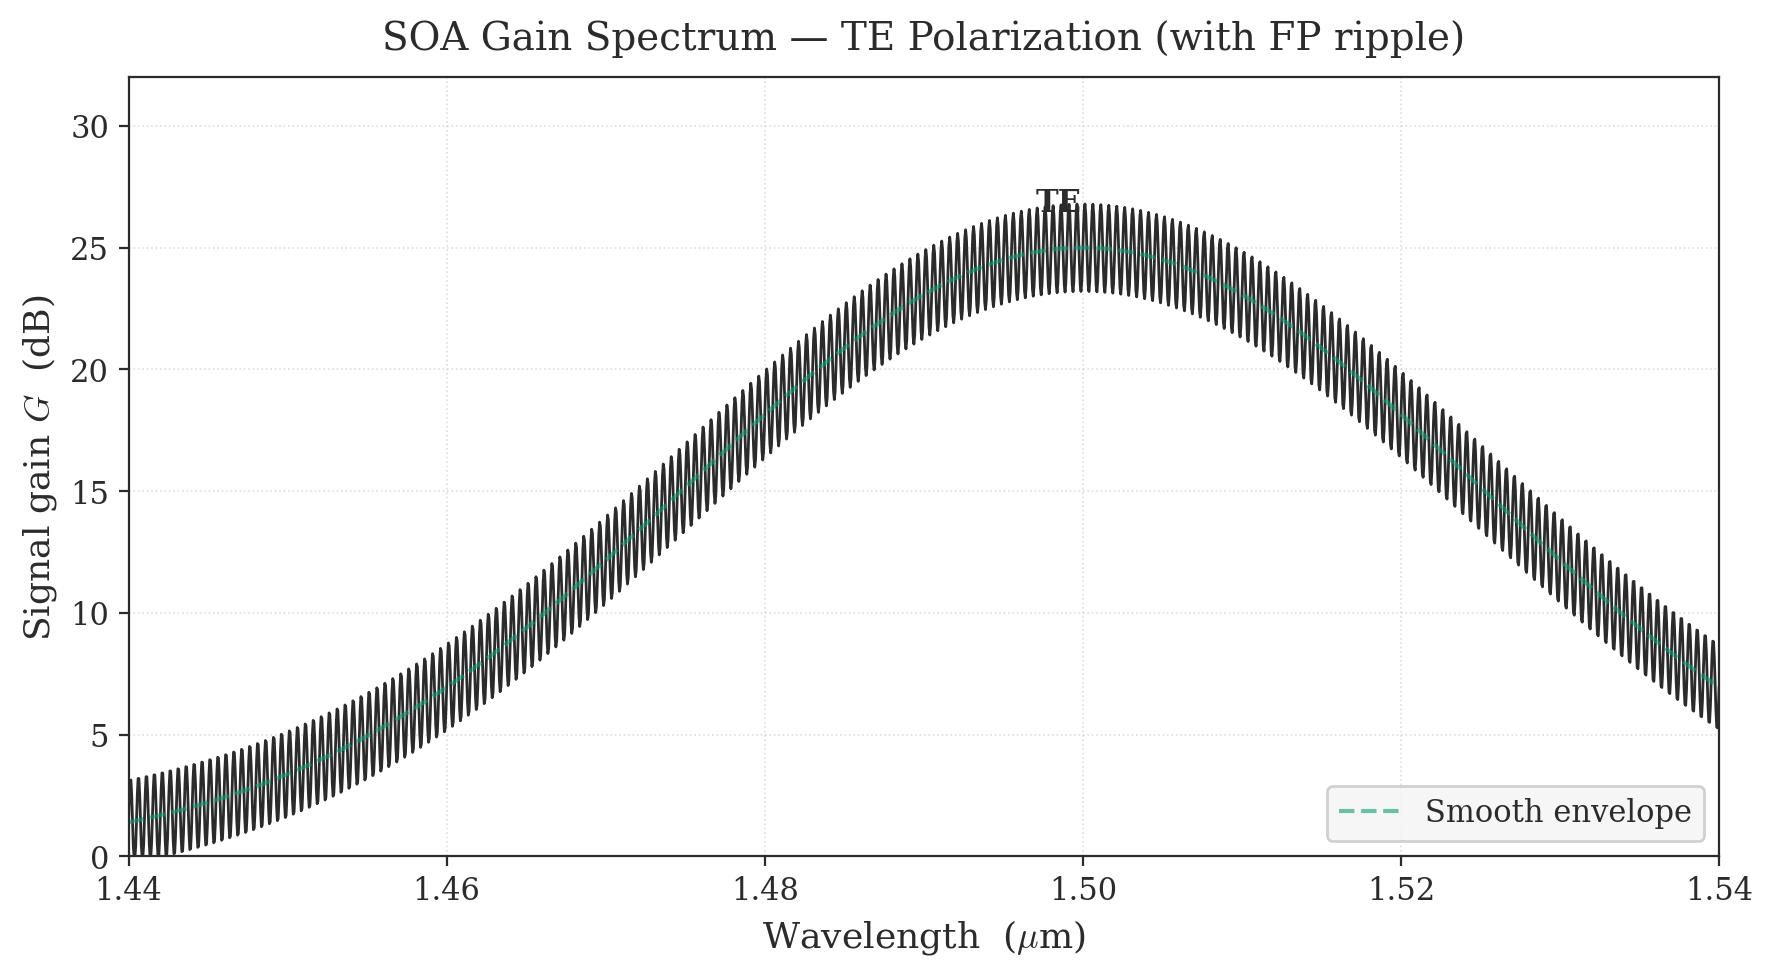
\includegraphics[width=0.6\textwidth]{Figures/Chapter 8/soa_gain_spectrum_te.jpg}
    \caption{SOA Gain Spectrum (TE polarization)}
    \label{fig:soa_gain_spectrum_te}
\end{figure}

must be kept below $\sim 3\,\text{dB}$ for broadband operation. This requires $G_0\sqrt{R_1R_2} < 0.17$, achieved by anti-reflection coatings reducing the facet reflectivities to below $R < 0.001$.

\begin{figure}[H]
    \centering
    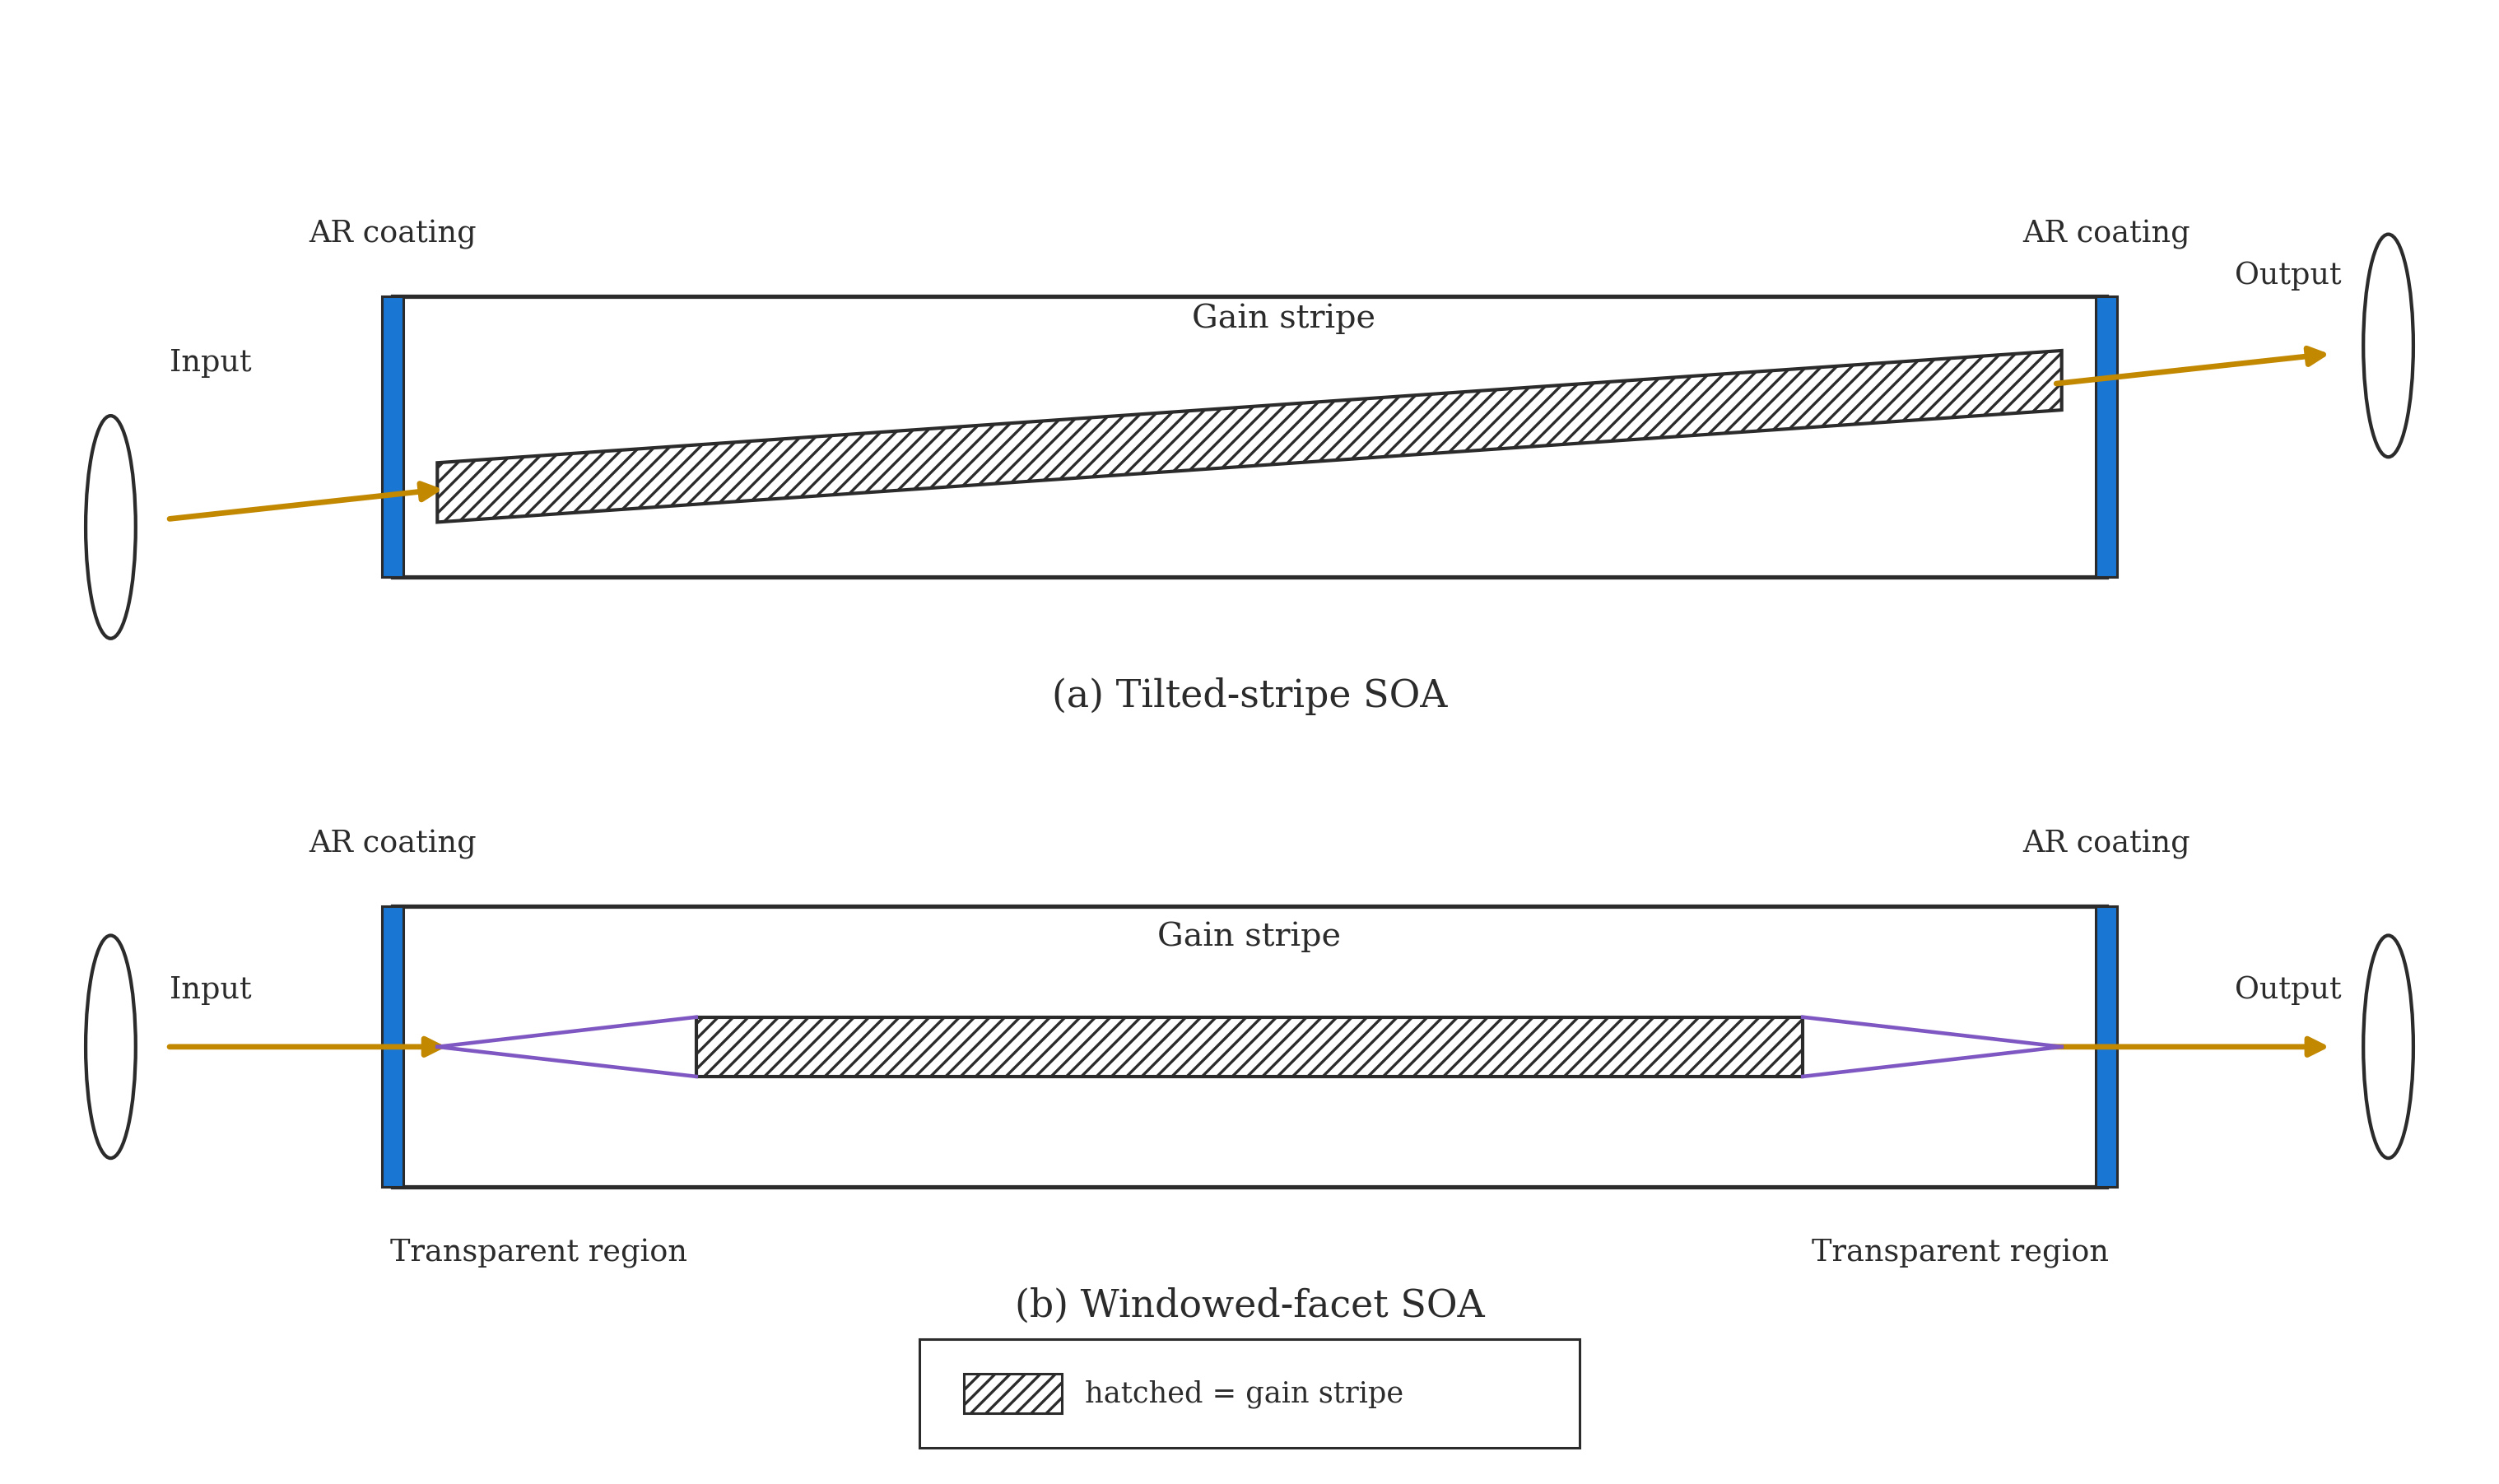
\includegraphics[width=0.7\textwidth]{Figures/Chapter 8/fabryperot_soa_geometries_tilted_vs_windowed_facets.jpg}
    \caption{Fabry-Perot SOA Geometries: Tilted vs. Windowed Facets}
    \label{fig:fabryperot_soa_geometries_tilted_vs_windowed_facets}
\end{figure}

% ------------------------------------------------------------------
\section{The Laser Diode: Static Characteristics}
% ------------------------------------------------------------------

\subsection{Lasing Conditions: Gain and Phase}

A laser diode is an SOA placed inside a Fabry-Pérot cavity formed by the cleaved semiconductor facets with reflectivities $R_1$ and $R_2$. Sustained oscillation requires the round-trip field to reproduce itself exactly in both amplitude and phase, which splits into two simultaneous conditions.

The \textbf{gain (amplitude) condition} requires the round-trip gain to exactly compensate the round-trip losses:
\begin{keyresult}
    \begin{equation}
        \Gamma\,g_\text{th} = \alpha + \alpha_m, \qquad \alpha_m = -\frac{1}{2L}\ln(R_1 R_2)
    \end{equation}
\end{keyresult}
where $\alpha$ is the distributed internal loss per unit length (free-carrier absorption, scattering) and $\alpha_m$ is the effective mirror loss — the distributed loss equivalent of the power that leaks out through the facets each round trip.

The \textbf{phase condition} selects discrete longitudinal modes:
\begin{equation*}
    2\beta L = 2m\pi \implies f_m = \frac{mc}{2nL}, \qquad m = 1, 2, 3, \ldots
\end{equation*}

These two conditions are structurally identical to the general laser oscillator threshold conditions — round-trip gain equals round-trip loss, and round-trip phase is an integer multiple of $2\pi$ — now expressed in terms of the semiconductor-specific parameters $\Gamma$, $g$, and the facet reflectivities.

\begin{figure}[H]
    \centering
    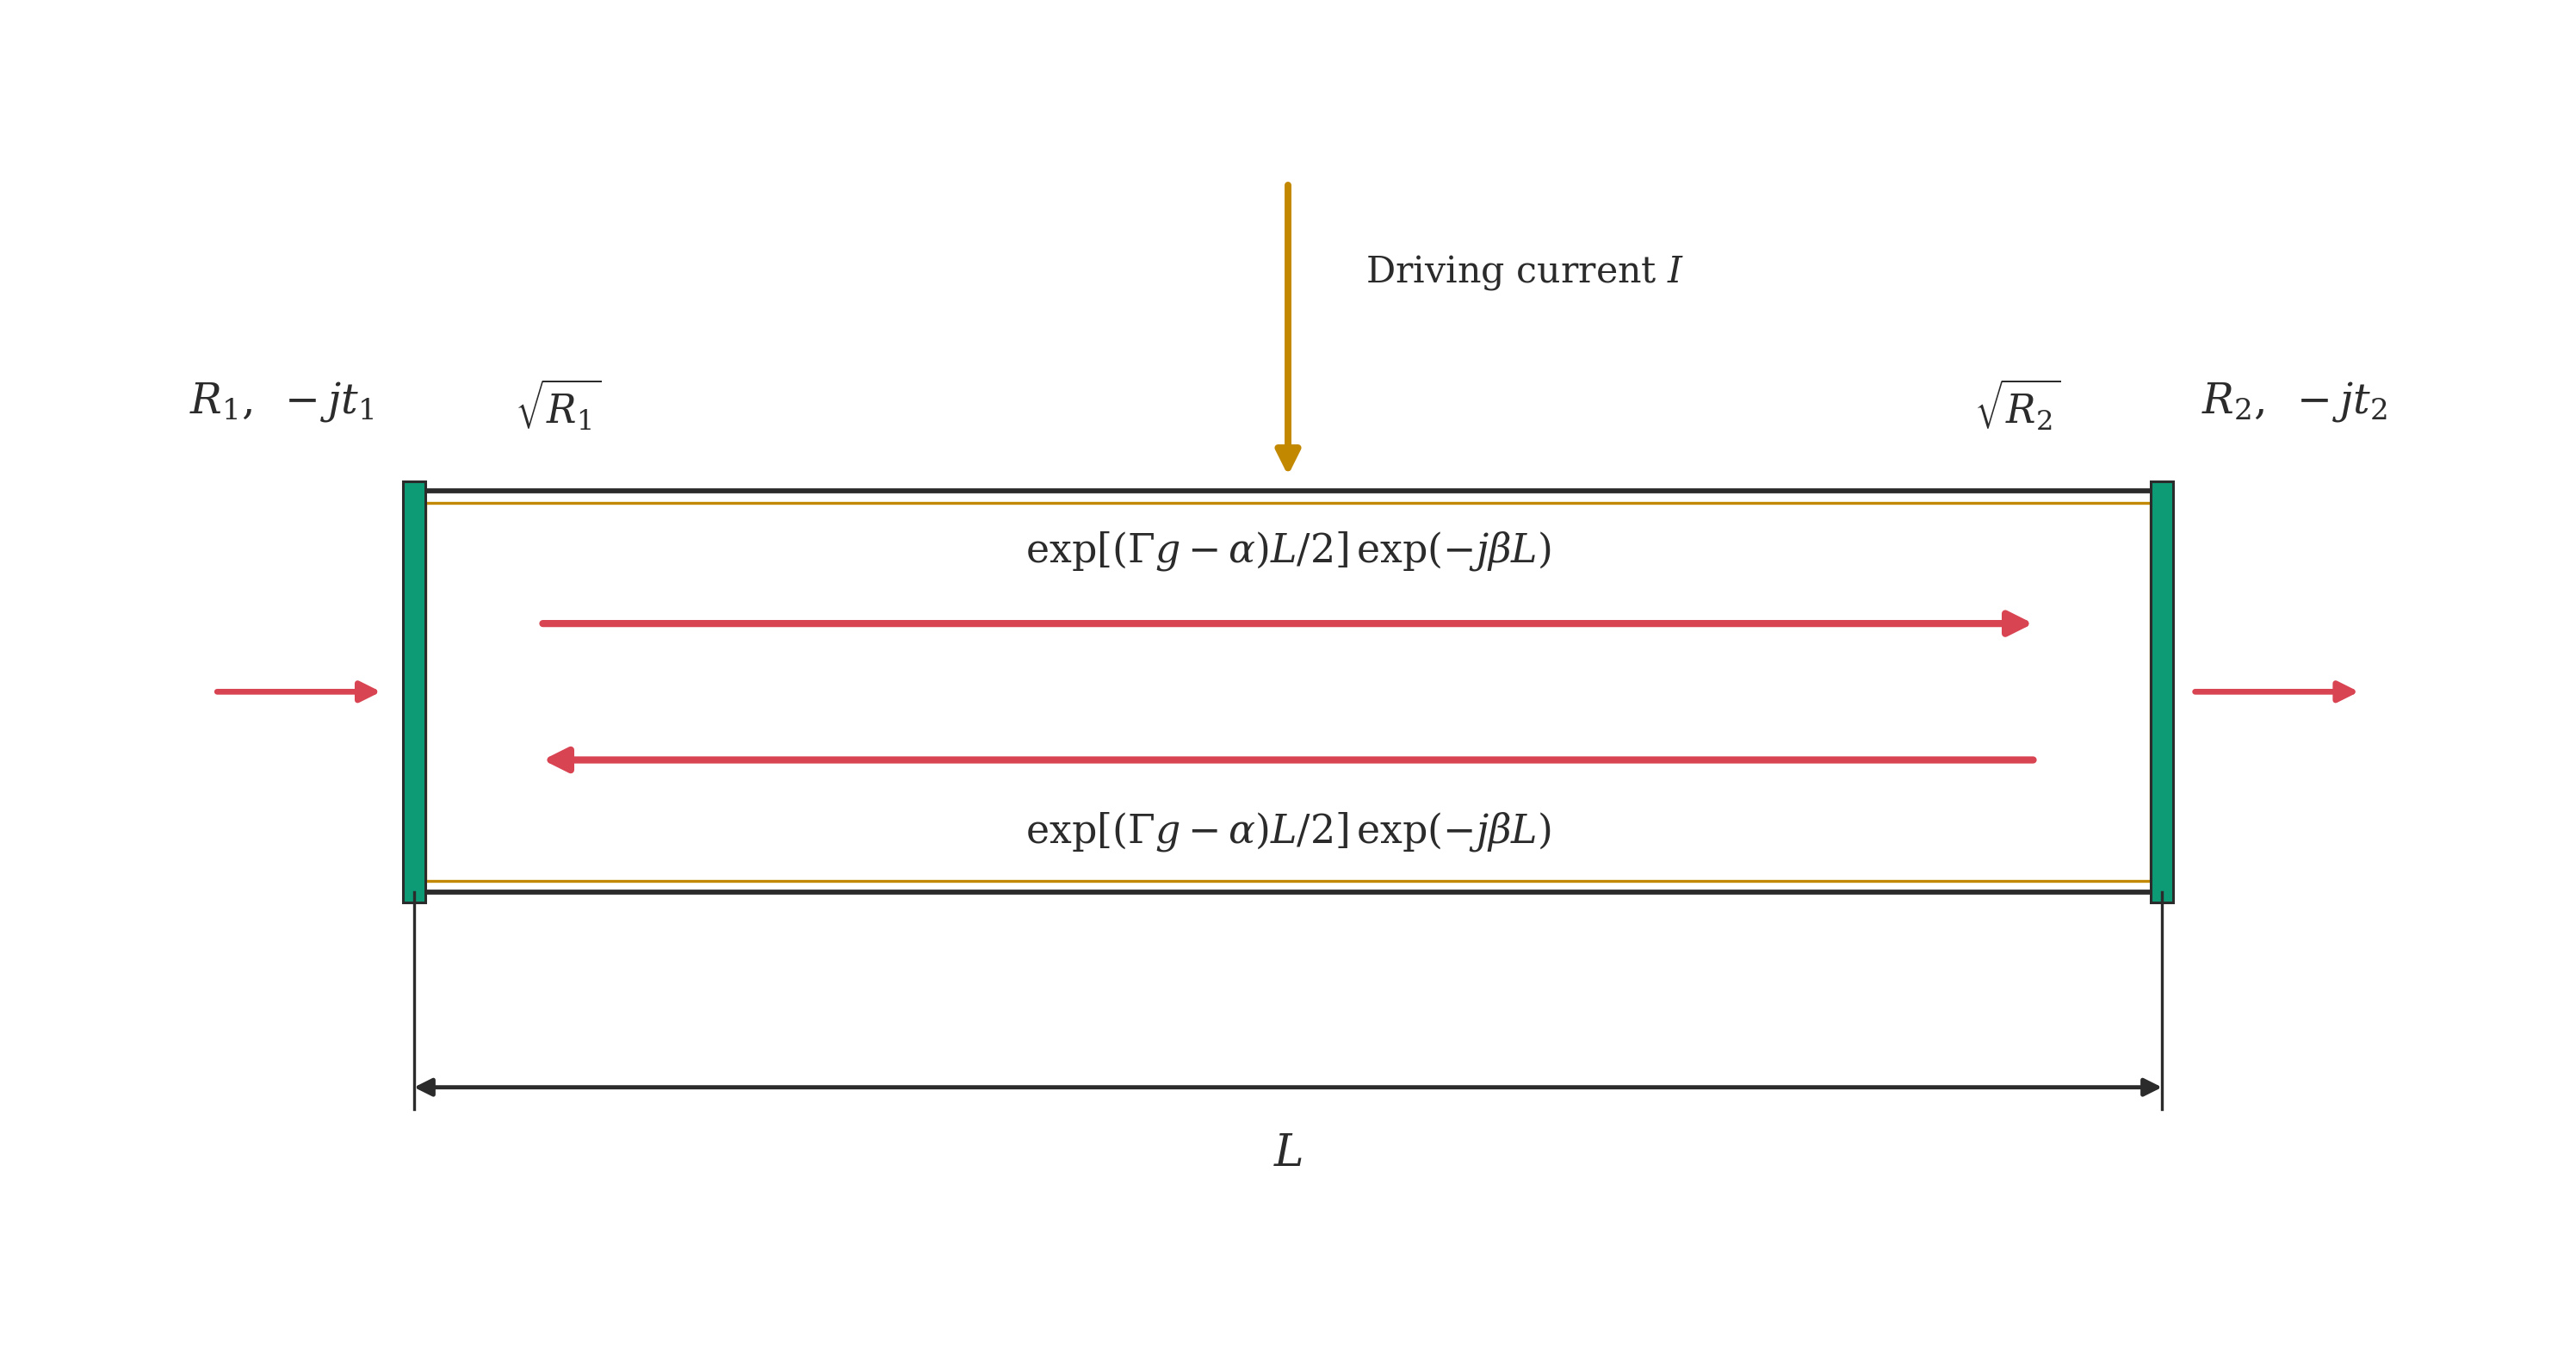
\includegraphics[width=0.6\textwidth]{Figures/Chapter 8/laser_diode_block_diagram_and_roundtrip_field.jpg}
    \caption{Laser Diode Block Diagram and Round-Trip Field}
    \label{fig:laser_diode_block_diagram_and_roundtrip_field}
\end{figure}

\subsection{Photon Lifetime}

The photon lifetime $\tau_{ph}$ quantifies the average time a photon survives inside the cavity before being lost to either internal absorption or mirror transmission. It follows from the round-trip loss analysis: after one round-trip time $\tau_{rt} = 2L/v_g$, the photon density is reduced by the factor $R_1 R_2 e^{-2\alpha L}$. Expanding for small fractional loss per round trip, the exponential decay rate is:
\begin{keyresult}
    \begin{equation}
        \frac{1}{\tau_{ph}} = v_g(\alpha + \alpha_m)
    \end{equation}
\end{keyresult}

The mirror loss $\alpha_m = -\ln(R_1 R_2)/(2L)$ contributes on equal footing with the internal loss — every photon has some probability of escaping through the facets on each round trip, and $\alpha_m$ quantifies that probability per unit length.

\subsection{Threshold Carrier Density and Threshold Current}

Using the linear gain model $g = B(N - N_\text{tr})$, the gain condition at threshold gives:
\begin{keyresult}
    \begin{equation}
        N_\text{th} = N_\text{tr} + \frac{1}{\Gamma B \tau_{ph}}
    \end{equation}
\end{keyresult}

Below threshold, the photon density is negligible and the carrier rate equation gives $N = J\tau/(ed)$. Setting $N = N_\text{th}$ determines the threshold current density:
\begin{keyresult}
    \begin{equation}
        J_\text{th} = \frac{ed}{\tau}\,N_\text{th} = \frac{ed}{\tau}\!\left(N_\text{tr} + \frac{1}{\Gamma B \tau_{ph}}\right)
    \end{equation}
\end{keyresult}

Every term in this expression has a physical handle: making $d$ smaller reduces the threshold current (less volume to invert), making $\Gamma$ larger reduces it (better mode-gain overlap), making $\tau_{ph}$ longer reduces it (lower loss cavity), and making $B$ larger reduces it (higher differential gain from the material).

\subsection{Below Threshold: LED-Like Behaviour}

Below the threshold current $I_\text{th}$, stimulated emission is negligible. The carrier density rises linearly with current, and the device emits broad-spectrum spontaneous light just like an LED:
\begin{equation*}
    N = \frac{J\tau}{ed}, \qquad S \approx 0
\end{equation*}

\begin{figure}[H]
    \centering
    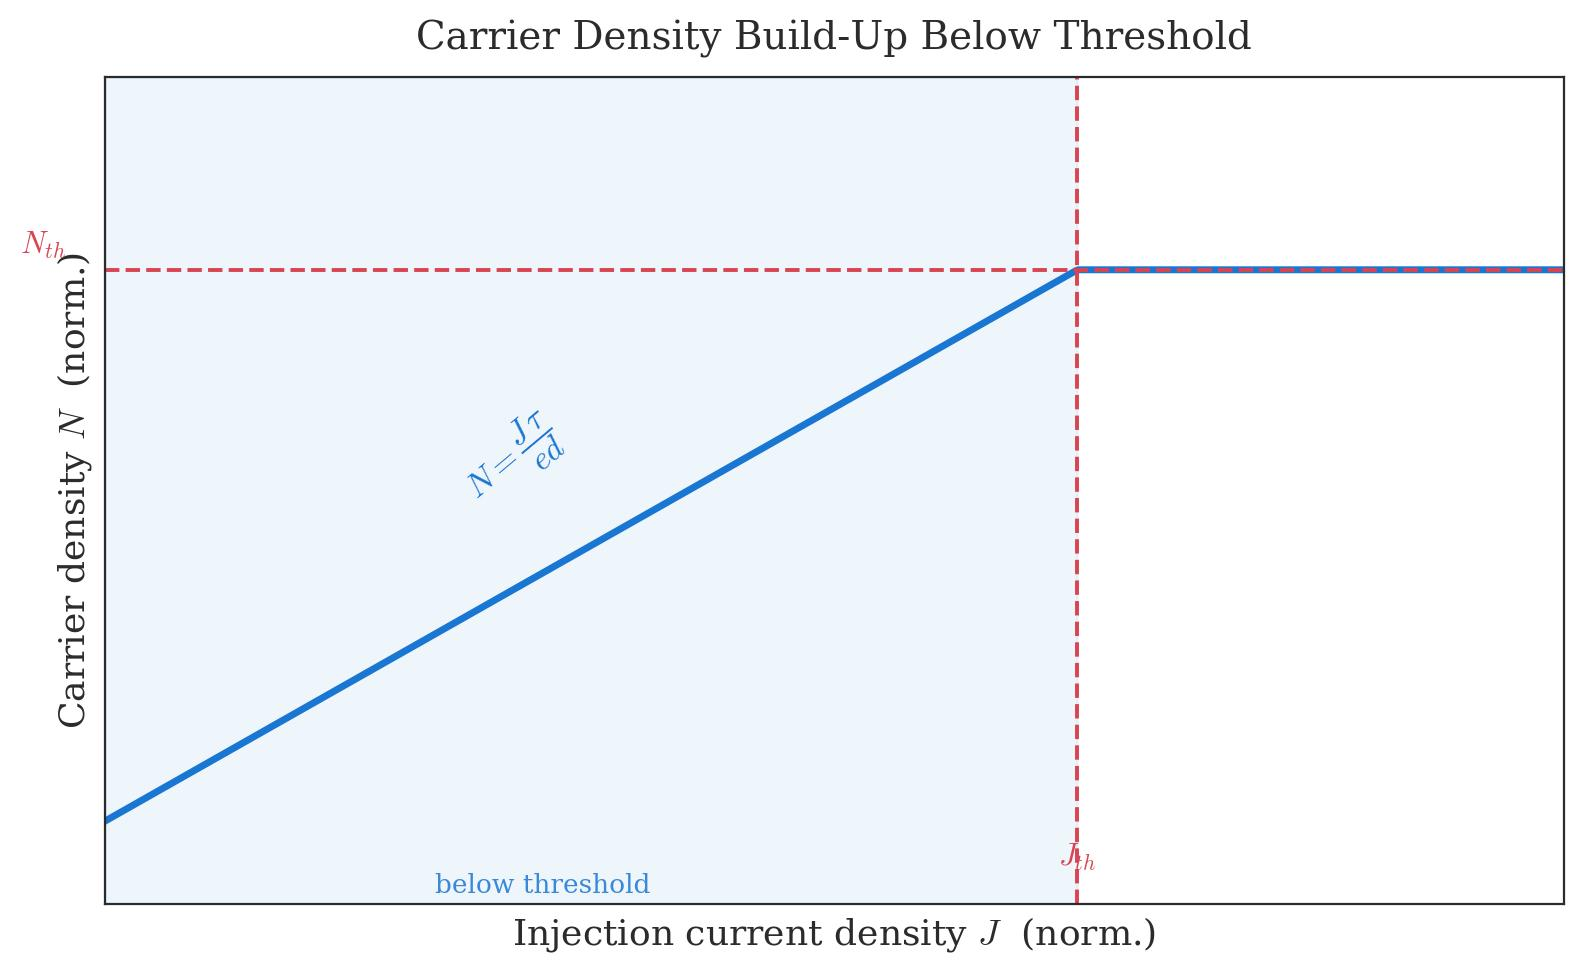
\includegraphics[width=0.6\textwidth]{Figures/Chapter 9/carrier_density_below_threshold.jpg}
    \caption{Carrier Density Below Threshold}
    \label{fig:carrier_density_below_threshold}
\end{figure}

The device is simply an LED with a cavity around it — the cavity does nothing useful below threshold, and the output is incoherent.

\subsection{Above Threshold: Carrier Clamping and the P--I Curve}

Above threshold, stimulated emission takes over. Any additional carriers injected beyond $N_\text{th}$ are almost instantly converted into coherent photons — the gain cannot rise above the threshold value without being immediately saturated back down by the growing photon density. This is carrier clamping: the same inversion-stabilising feedback that we saw in any saturated gain medium, now playing out inside the laser diode cavity. The carrier density is pinned:
\begin{equation*}
    N \approx N_\text{th} \quad (I > I_\text{th})
\end{equation*}

Substituting $N = N_\text{th}$ into the steady-state photon rate equation ($dS/dt = 0$) and solving for $S$:
\begin{keyresult}
    \begin{equation}
        S = \frac{\tau_{ph}}{ed}(J - J_\text{th}) + \beta\,\frac{\tau_{ph}}{\tau_r}\,N_\text{th}
    \end{equation}
\end{keyresult}

The first term is the dominant above-threshold contribution — every increment of current above $J_\text{th}$ goes directly into the photon field. The second term is the small spontaneous emission seeding the lasing mode (characterised by the spontaneous emission coupling factor $\beta$), which is usually negligible in edge-emitting laser diodes where $\beta \ll 1$.

\begin{figure}[H]
    \centering
    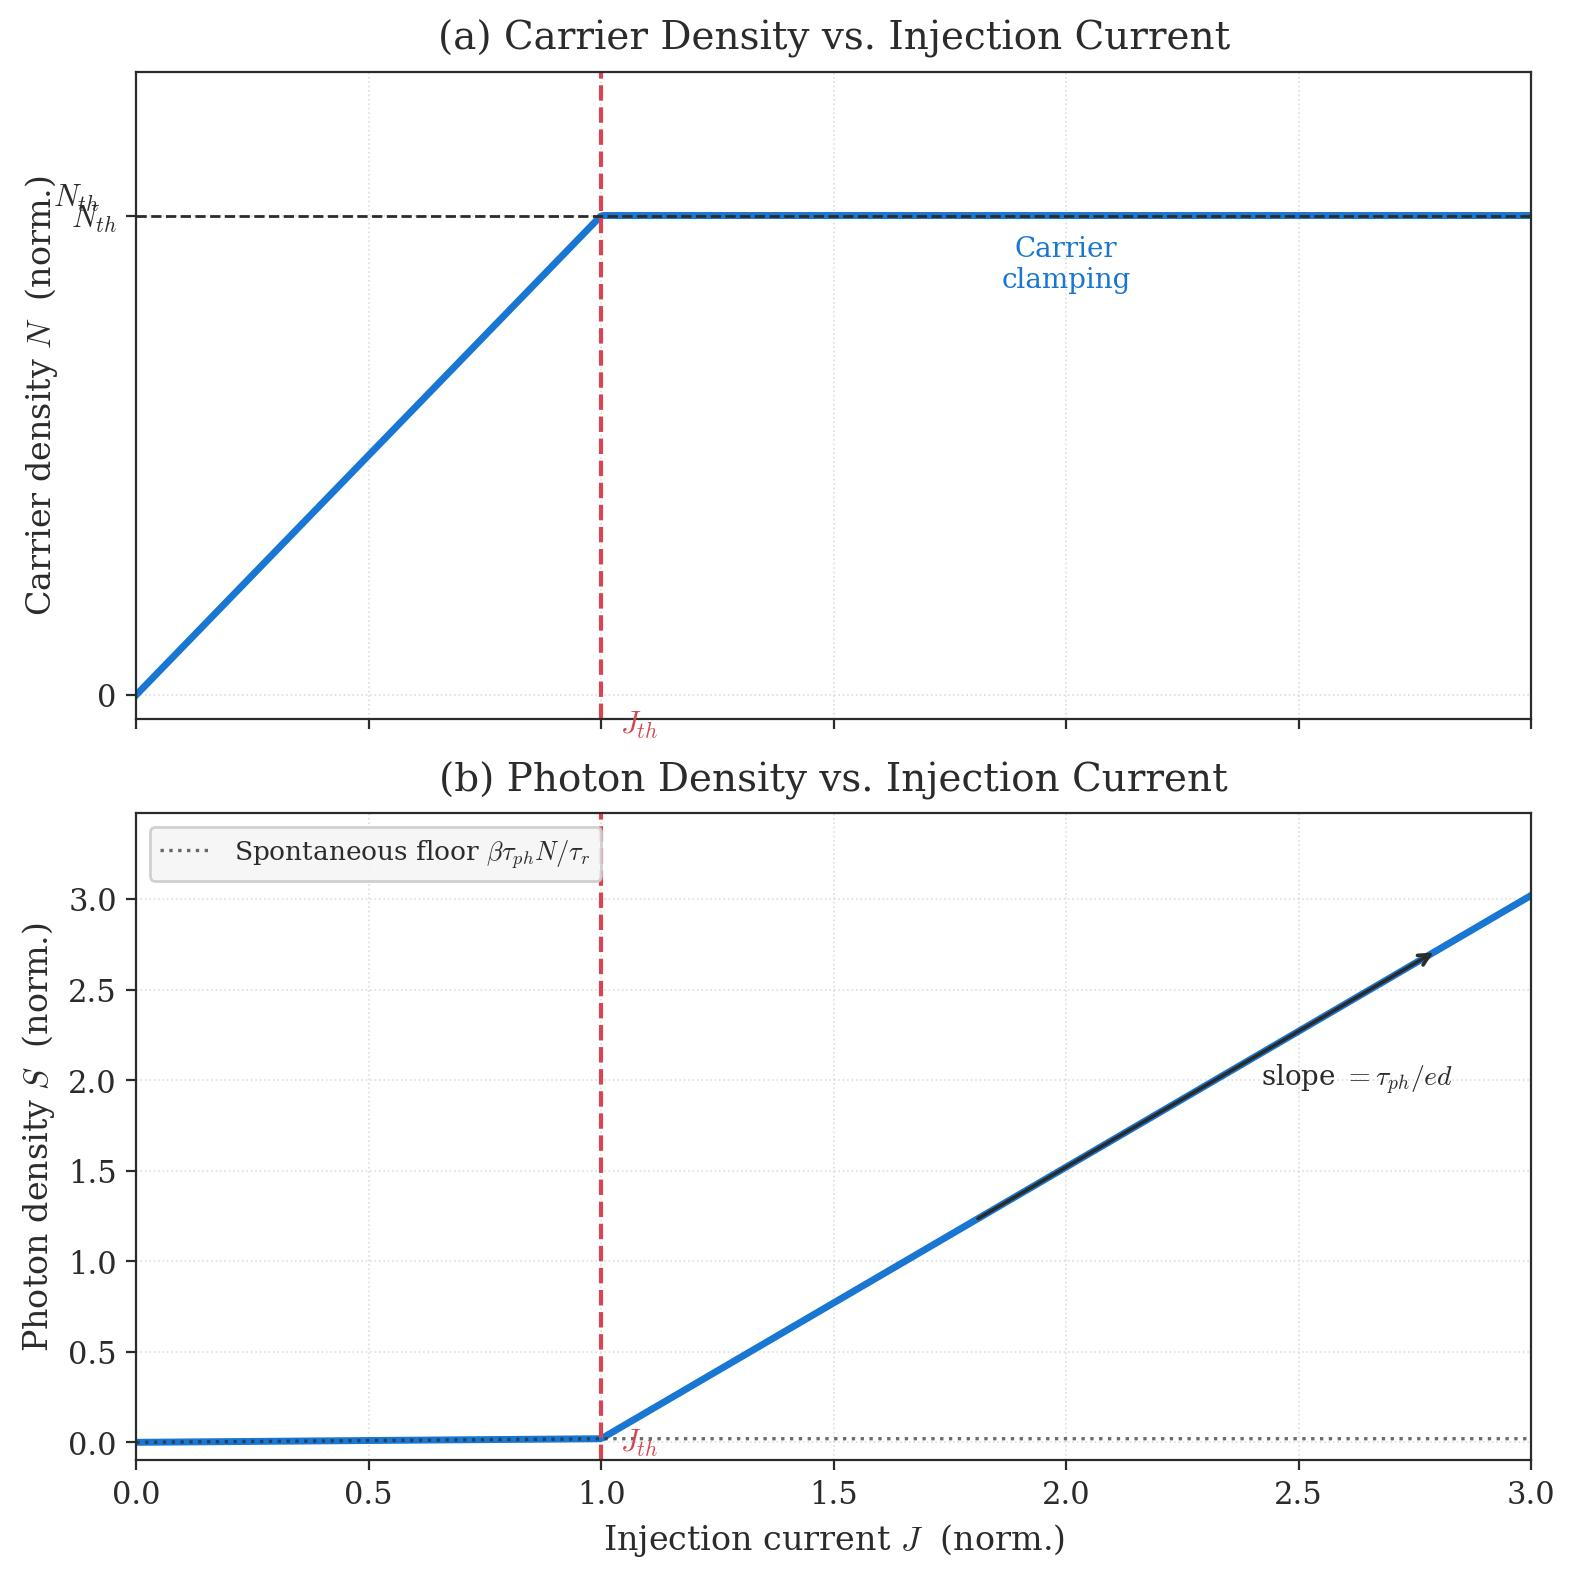
\includegraphics[width=0.7\textwidth]{Figures/Chapter 8/ld_dc_characteristics.jpg}
    \caption{Laser Diode DC Characteristics: $N$ and $S$ vs. Current}
    \label{fig:ld_dc_characteristics}
\end{figure}

To derive the output power through facet $R_1$, we relate it to the rate of photon generation. Above threshold, the carrier density is clamped at $N_\text{th}$, so any additional injected current above $I_\text{th}$ is converted into photons by stimulated emission. The rate of photon generation in the cavity is:
\begin{equation*}
    \left.\frac{d N_p}{dt}\right|_\text{stim} = \frac{I - I_\text{th}}{e}
\end{equation*}
The generated photons decay at rate $1/\tau_{ph} = v_g(\alpha + \alpha_m)$. The fraction of photons that escape the cavity through the mirrors (mirror loss) rather than being absorbed internally is:
\begin{equation*}
    \eta_\text{mirror} = \frac{\alpha_m}{\alpha + \alpha_m} = v_g \alpha_m \tau_{ph}
\end{equation*}
So the total rate of photons escaping the cavity from both mirrors is $\eta_\text{mirror} \frac{I - I_\text{th}}{e}$. The mirror loss coefficient $\alpha_m$ is the sum of the losses from mirror 1 and mirror 2:
\begin{equation*}
    \alpha_m = \alpha_{m1} + \alpha_{m2} = \frac{1}{2L}\ln\!\left(\frac{1}{R_1}\right) + \frac{1}{2L}\ln\!\left(\frac{1}{R_2}\right)
\end{equation*}
The fraction of escaping photons that exit specifically through mirror 1 is $F_1 = \alpha_{m1}/\alpha_m$. Multiplying the photon generation rate, the escape fraction, the mirror 1 fraction, and the photon energy $h\nu$ yields the output power:
\begin{align*}
    P_\text{out} &= h\nu \cdot F_1 \cdot \eta_\text{mirror} \cdot \left(\frac{I - I_\text{th}}{e}\right) \\
    &= h\nu \left( \frac{\frac{1}{2L}\ln(1/R_1)}{\alpha_m} \right) (v_g \alpha_m \tau_{ph}) \left(\frac{I - I_\text{th}}{e}\right) \\
    &= \left( \frac{1}{2L}\ln\!\frac{1}{R_1} \cdot \frac{h\nu v_g \tau_{ph}}{e} \right) (I - I_\text{th})
\end{align*}
Thus, the output power through facet $R_1$ is:
\begin{equation*}
    P_\text{out} \approx \eta_d\,(I - I_\text{th})
\end{equation*}
where the \textbf{slope efficiency} (or differential efficiency) is:
\begin{keyresult}
    \begin{equation}
        \eta_d = \frac{1}{2L}\ln\!\frac{1}{R_1}\cdot\frac{h\nu v_g \tau_{ph}}{e}
    \end{equation}
\end{keyresult}

\begin{figure}[H]
    \centering
    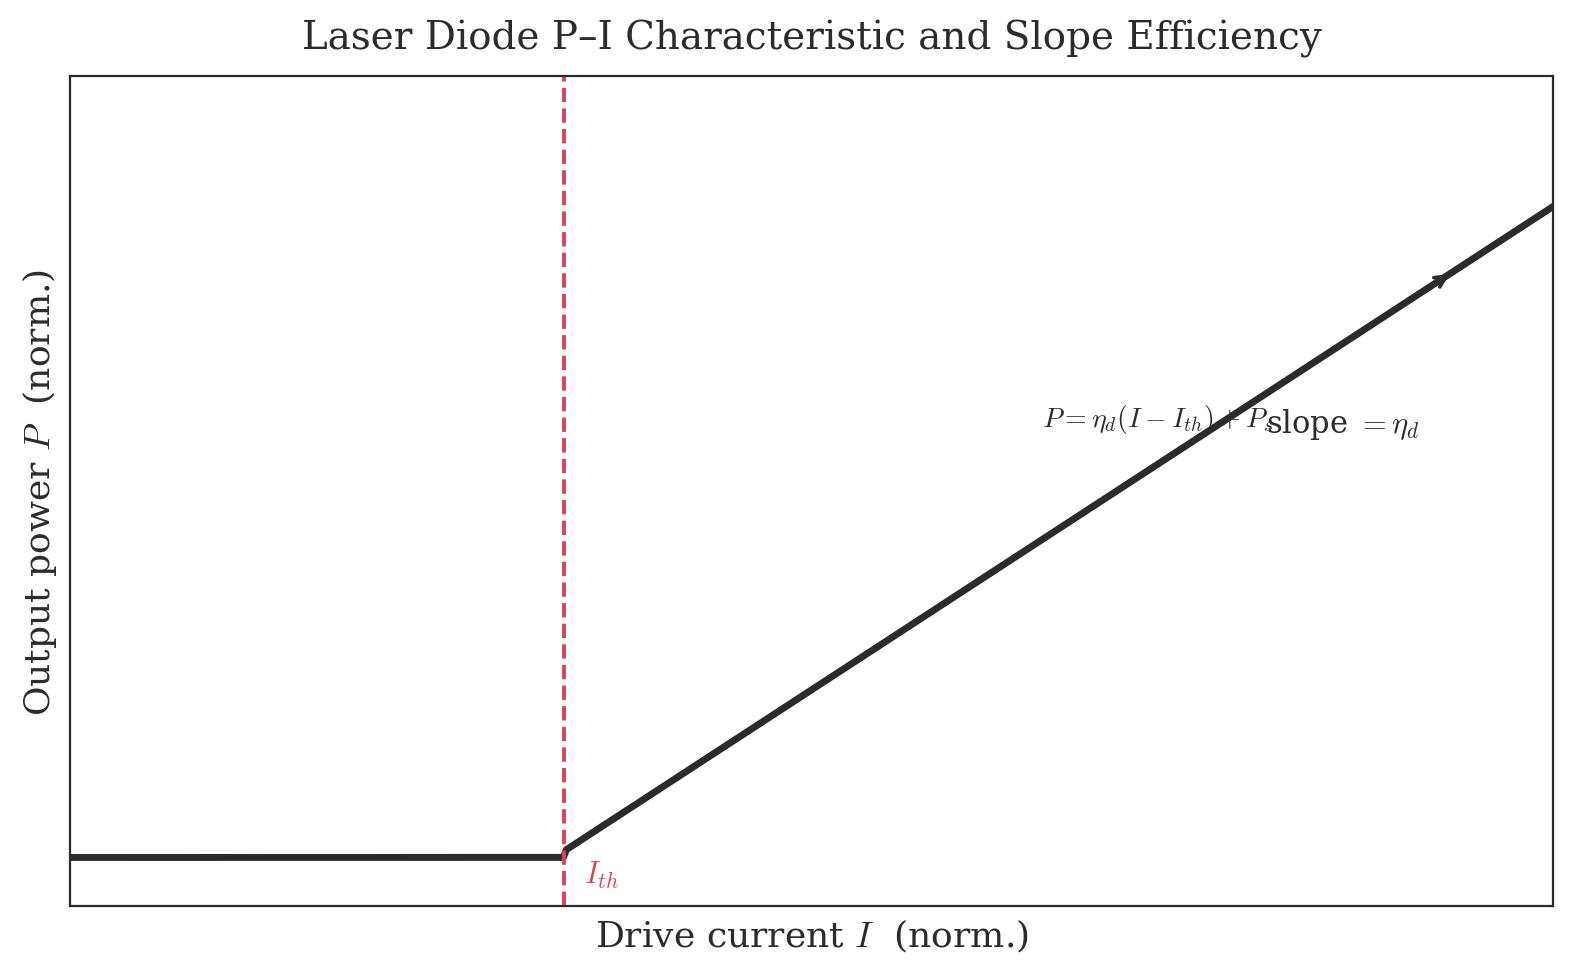
\includegraphics[width=0.6\textwidth]{Figures/Chapter 9/ld_pi_characteristic.jpg}
    \caption{Laser Output Power vs. Drive Current}
    \label{fig:ld_pi_characteristic}
\end{figure}

This linear above-threshold P--I relationship — with its sharp kink at $I_\text{th}$ — is the defining characteristic of every laser diode. Measuring the kink and the slope gives $I_\text{th}$ and $\eta_d$ directly, the two most important DC performance parameters.

\subsection{Temperature Dependence}

Temperature degrades both the threshold current and the slope efficiency. The empirical characterisation commonly used is:
\begin{equation*}
    I_\text{th}(T) = I_\text{th}(T_\text{ref})\exp\!\left(\frac{T - T_\text{ref}}{T_0}\right)
\end{equation*}
\begin{equation*}
    \eta_d(T) = \eta_d(T_\text{ref})\exp\!\left(-\frac{T - T_\text{ref}}{T_1}\right)
\end{equation*}

\begin{figure}[H]
    \centering
    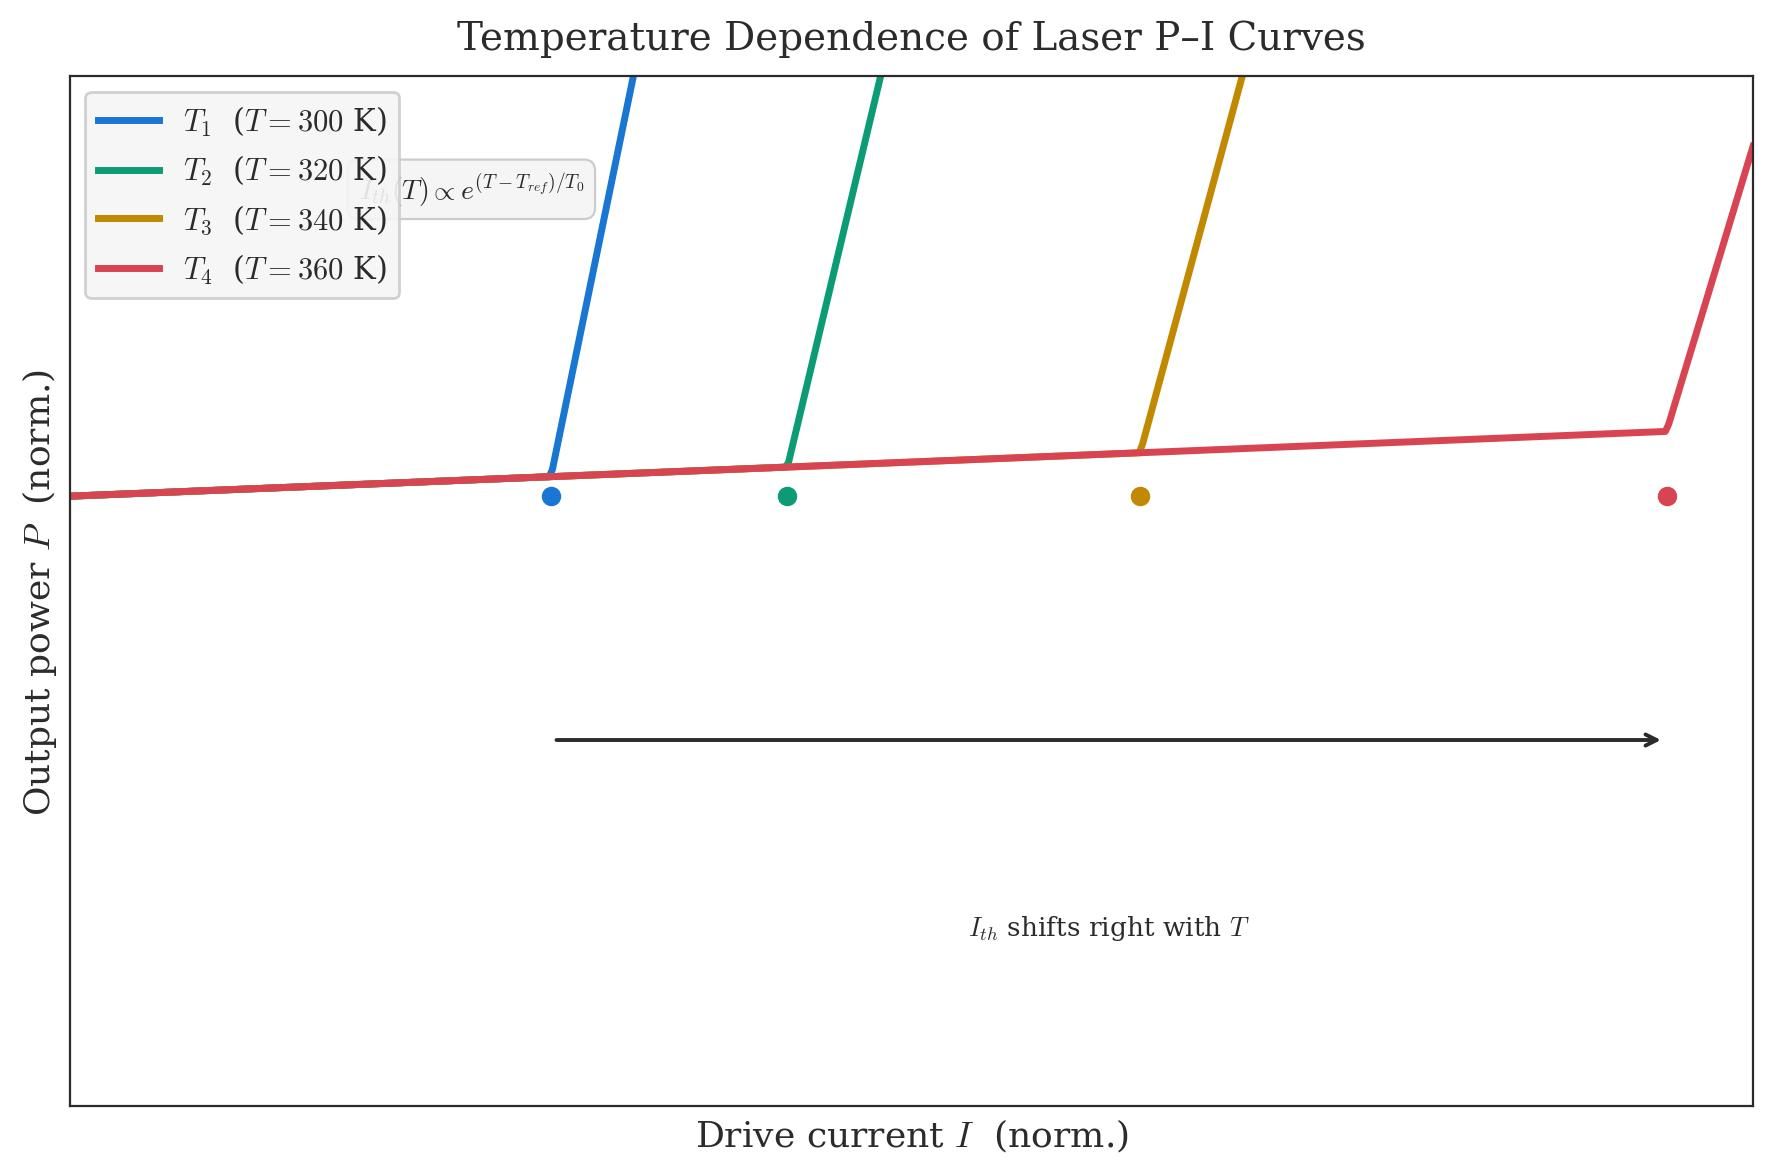
\includegraphics[width=0.6\textwidth]{Figures/Chapter 9/ld_pi_temperature.jpg}
    \caption{Temperature Dependence of the Laser P–I Curves}
    \label{fig:ld_pi_temperature}
\end{figure}

where $T_0$ (the characteristic temperature) quantifies threshold sensitivity to temperature — a higher $T_0$ means the threshold rises more slowly with temperature, which is desirable. At a fixed drive current, the P--I curve shifts right (higher threshold) and flattens (lower slope) as temperature rises. This is why high-power laser modules require thermoelectric coolers to stabilise the junction temperature.

% ------------------------------------------------------------------
\section{From Static Behaviour to Dynamics}
% ------------------------------------------------------------------

The DC picture of the laser diode we have built here — threshold, carrier clamping, and the linear P--I curve — explains the static behaviour beautifully. However, a laser diode used in a communications system is never just sitting at DC. The data stream modulates the drive current at gigabit-per-second rates, and the laser must respond faithfully to every current fluctuation.

\begin{keyinsight}[The Limitation of Static Analysis]
    The DC analysis treats the coupled carrier-photon system as if it were always in steady state. This works perfectly for calculating threshold currents and slope efficiencies, but it completely misses two critical dynamic effects:

    First, the laser cannot respond instantaneously to a current step — there is a \textbf{turn-on delay} while the carrier density builds from its initial value up to the threshold. This limits how quickly the device can be switched.

    Second, after turn-on, the carrier and photon densities do not immediately settle to their new steady-state values. They overshoot, undershoot, and ring at a characteristic frequency before equilibrating. These \textbf{relaxation oscillations} limit the modulation bandwidth and introduce pattern-dependent distortion in high-speed data links.

    Both phenomena are invisible to the DC rate equation but emerge naturally from the coupled carrier-photon dynamics when we solve the full time-dependent system.
\end{keyinsight}

The next chapter will linearise the coupled rate equations around the above-threshold bias point, derive the small-signal modulation transfer function, extract the relaxation oscillation frequency and the damping factor, and then analyse the large-signal turn-on delay — completing the dynamic picture of the laser diode and connecting it to single-frequency architectures like the DFB and DBR laser.
